\documentclass[9pt]{beamer}
%\documentclass[9pt,aspectratio=169]{beamer}
\usepackage[utf8]{inputenc}
\usepackage[english]{babel}
\usepackage[T1]{fontenc}
\usepackage{tikz}
\usepackage{times}
\usefonttheme[onlymath]{serif} 
\usepackage{etoolbox}
\usepackage{xcolor}
\usepackage{amsmath}
\usepackage{graphicx}
\usepackage{pdfpages}
\usepackage{eurosym}
\usepackage[absolute,overlay]{textpos}
\usepackage{animate}
\usepackage{textcomp}
\usepackage{booktabs}
\usepackage{verbatim}
\usepackage{biblatex}
\usepackage{tikz}
\usepackage{media9}
\addbibresource{dlpbibli.bib}

% Defining new colors
\definecolor{DarkGreen}{rgb}{0.0, 0.65, 0.31}
\definecolor{NewRed}{rgb}{0.89, 0.02, 0.17}


\usetheme{ARMINES}

\author[Daniella LOPES PINTO]{Daniella LOPES PINTO \textsuperscript{1,2*} \\ 
\texttt{\textcolor{black}{daniella.lopes\_pinto@minesparis.psl.eu}}}
\subtitle{\LARGE Finite element models for the study of hydrogen embrittlement of steel structures}

\institute
{\textbf{Thesis director}: Jacques BESSON \textsuperscript{1} \\
\vspace{0.25cm}
\textbf{Industrial advisor}: Nikolay OSIPOV \textsuperscript{2} \\
\vspace{0.4cm}
{\textsuperscript{1} Centre des Matériaux, Mines Paris} \\
\vspace{0.15cm}
\textsuperscript{2} Transvalor S.A. \\
\vspace{0.2cm}
\center{\textbf{Thesis defense} \\ \small March 7\textsuperscript{th} 2025} 
\center{\textcolor{white}{XXXXXXXX}}}


\begin{document}

\begin{frame}[plain]
    \maketitle
\end{frame}

\section{Introduction}

%%%%%%%%%%%%%%%%%%%%%%%%%%%%%%%%%%%%%%%%%%%%%%%%%%%%%%%%%%%

\begin{frame}{Background and challenges}

    \begin{itemize}
		\item In the context of \textbf{energy transition}, \textbf{hydrogen} plays an important role as an \textbf{energy vector}
		\vspace{0.15cm}
		\item Hydrogen can be produced from other \textbf{renewable sources}, such as wind and solar
		\vspace{0.15cm}
		\item Hydrogen transport using \textbf{existing natural gas pipelines} (40,000 km in France, \texteuro 50 billion in assets, up to 80 years old) is a proposal for hydrogen transport
    \end{itemize}
    
    \vspace{0.2cm}

\begin{figure}
	\centering
	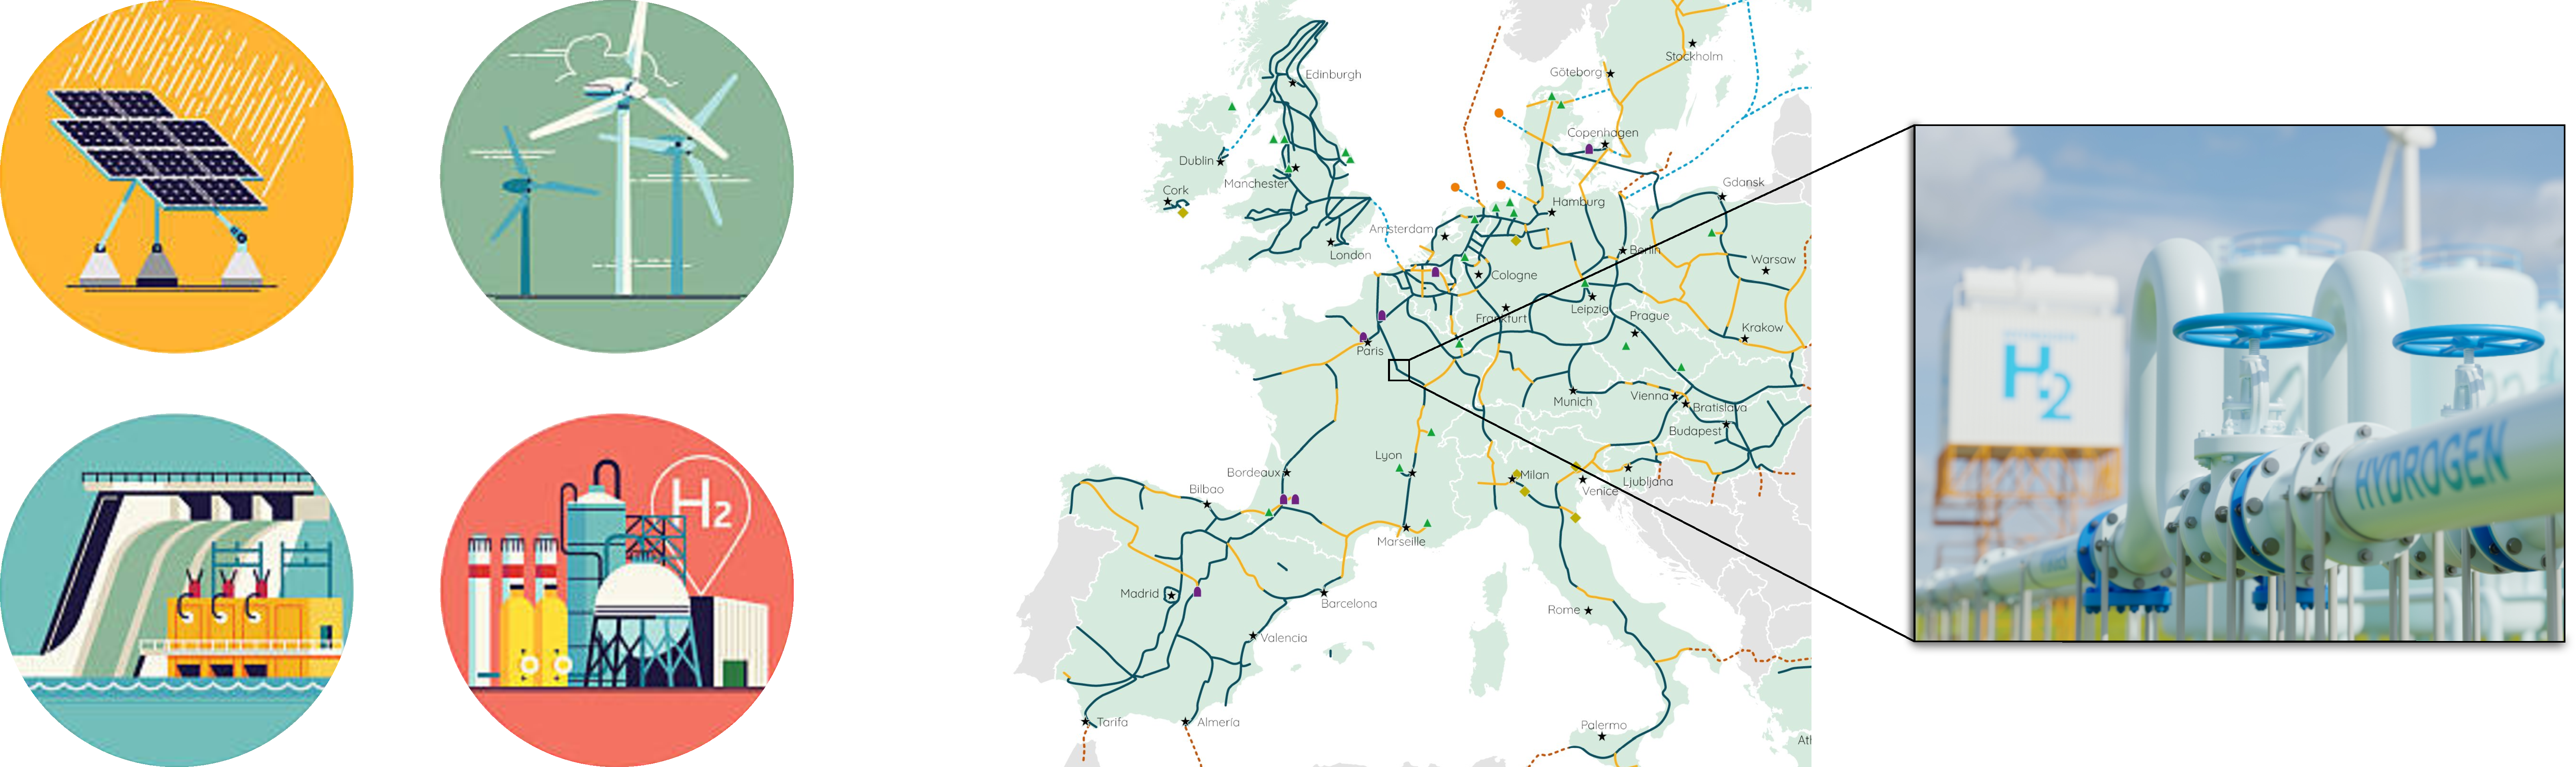
\includegraphics[width=0.92\textwidth]{Images/Context.pdf}
\end{figure}
    
\end{frame}

%%%%%%%%%%%%%%%%%%%%%%%%%%%%%%%%%%%%%%%%%%%%%%%%%%%%%%%%%%%

\begin{frame}{Background and challenges}

\begin{itemize}
	\item The steels used in gas pipelines are typically susceptible to \textbf{hydrogen embrittlement}
	\vspace{0.15cm}
	\item Hydrogen embrittlement: ductility and toughness reduction, premature failure
	\vspace{0.15cm}
	\item Measure material properties from \textbf{small samples} without service interruption
\end{itemize}

\vspace{0.15cm}

\begin{figure}
	\centering
	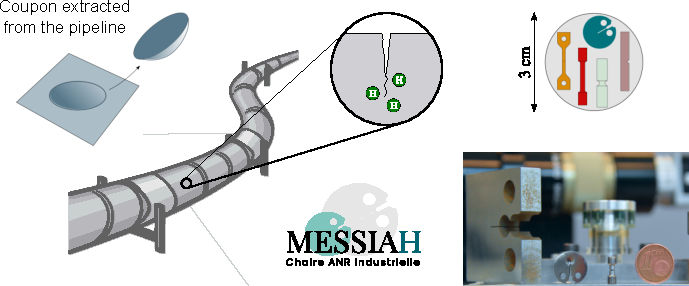
\includegraphics[width=0.95\textwidth]{Images/MESSIAH.pdf}
\end{figure}

\end{frame}

%%%%%%%%%%%%%%%%%%%%%%%%%%%%%%%%%%%%%%%%%%%%%%%%%%%%%%%%%%%

\begin{frame}{Background and challenges}

\begin{itemize}
    \item Transferability from sub-size specimens to a full scale structure $\rightarrow$ \textbf{Specimen size significantly influences toughness}
    \vspace{0.15cm}
    \item Beyond a critical thickness, toughness becomes relatively insensitive to further increases
\end{itemize}

\begin{figure}
    \centering
    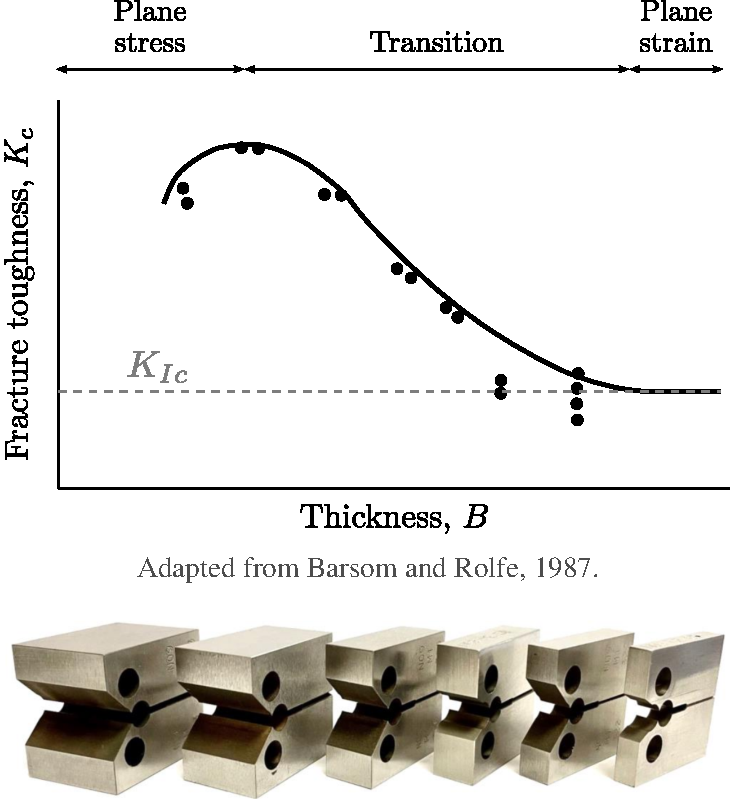
\includegraphics[width=0.75\textwidth]{Images/plateau_plane_strain.pdf}
\end{figure}


\end{frame}

%%%%%%%%%%%%%%%%%%%%%%%%%%%%%%%%%%%%%%%%%%%%%%%%%%%%%%%%%%%

\begin{frame}{Main objectives}

\begin{itemize}
    \item \textbf{Hydrogen embrittlement:}
    \vspace{0.2cm}
    \begin{itemize}
    	\item Develop a model coupling plasticity, damage, and hydrogen diffusion
    	\vspace{0.2cm}
    	\item Reproduce the degradation of the material’s mechanical properties, ductility and toughness loss, multi-crack initiation
    \end{itemize}
    
    \vspace{0.2cm}
    
    \item \textbf{Fracture toughness simulations:}

	\vspace{0.2cm}    
    
    \begin{itemize}
    	\item Analyze the effect of the specimen's size and thickness on fracture toughness through numerical simulations
    \end{itemize}
    
    \vspace{0.2cm}
   	\item \textbf{Validate the model against experimental data}
\end{itemize}

\vspace{3.25cm}

	\begin{tikzpicture}[remember picture, overlay]
    	\node at (current page.south west) [xshift=3cm, yshift=2.25cm] {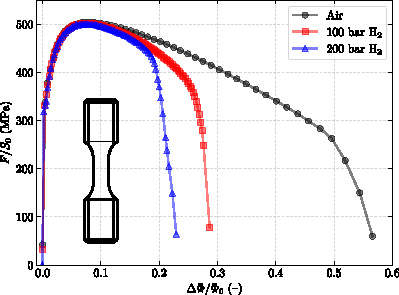
\includegraphics[width=4.5cm]{Images/tensile_test.pdf}}; 
    \end{tikzpicture}
    
	\begin{tikzpicture}[remember picture, overlay]
    	\node at (current page.south west) [xshift=9cm, yshift=1.8cm] {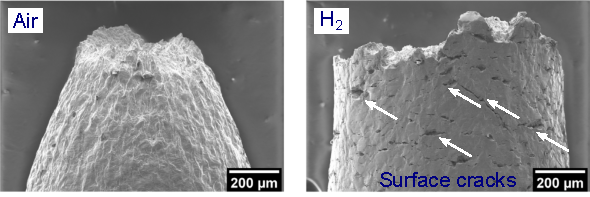
\includegraphics[width=5.5cm]{Images/fracture_surface_2.pdf}}; 
    \end{tikzpicture}
    
	\begin{tikzpicture}[remember picture, overlay]
    	\node at (current page.south west) [xshift=10.5cm, yshift=4cm] {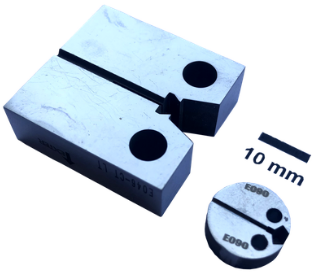
\includegraphics[width=2.5cm]{Images/CT_mDCT.png}}; 
    \end{tikzpicture}

% Say that this model not only allows the prediction of hydrogen assisted failure, but also to estimate the hydrogen distribution during loading and it can help interpreting experiments
% Add figures and animations from TISD ?

\end{frame}

%%%%%%%%%%%%%%%%%%%%%%%%%%%%%%%%%%%%%%%%%%%%%%%%%%%%%%%%%%%

\begin{frame}{Outline}
    \tableofcontents
\end{frame}

%%%%%%%%%%%%%%%%%%%%%%%%%%%%%%%%%%%%%%%%%%%%%%%%%%%%%%%%%%%%

\section{Hydrogen inside metals}

\begin{frame}{Outline}
	\tableofcontents[ 
    currentsubsection, 
    hideothersubsections, 
    sectionstyle=show/shaded, 
    subsectionstyle=show/shaded, 
    ] 
\end{frame}

%%%%%%%%%%%%%%%%%%%%%%%%%%%%%%%%%%%%%%%%%%%%%%%%%%%%%%%%%%%

\begin{frame}{Hydrogen uptake}

\begin{itemize}
	\item \textbf{Sieverts' law:} The solubility of a diatomic gas in a metal is proportional to the square root of the gas pressure
\end{itemize}

\vspace{1cm}

    \begin{minipage}{0.55\textwidth}
        \centering
        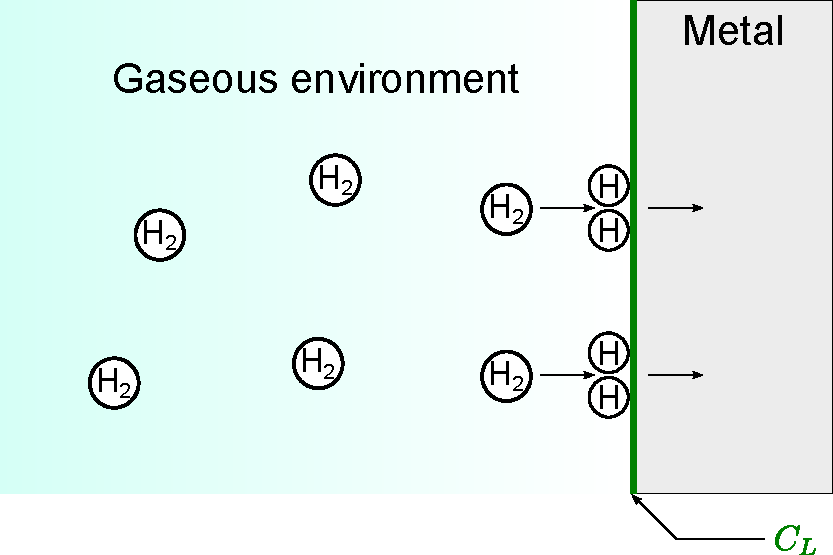
\includegraphics[width=\textwidth]{Images/H2_uptake.pdf}
    \end{minipage}
    \hfill
    \begin{minipage}{0.42\textwidth}
        \centering
        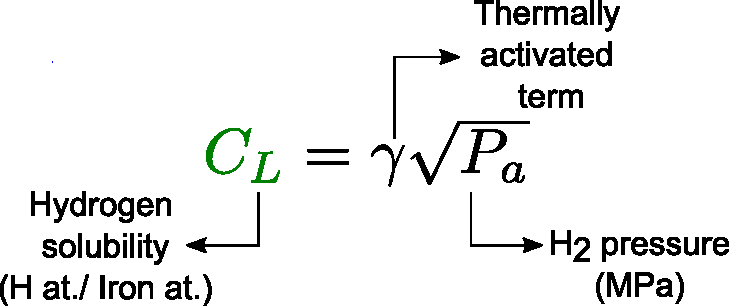
\includegraphics[width=\textwidth]{Images/sieverts.pdf}
    \end{minipage}

\end{frame}

%%%%%%%%%%%%%%%%%%%%%%%%%%%%%%%%%%%%%%%%%%%%%%%%%%%%%%%%%%%

\begin{frame}{Hydrogen diffusion and trapping}

    \begin{columns}
    
        \begin{column}{0.8\textwidth}
    
            \begin{itemize}
                \item Model from \textcolor{darkgray}{Sofronis and McMeeking (1989)} and corrected by \textcolor{darkgray}{Krom \textit{et al.} (1999)}
                
                \vspace{0.35cm}
            
                \item \textbf{Hydrogen concentration:} \hspace{0.5cm} $ \displaystyle C = \textcolor{DarkGreen}{C_L} + \textcolor{blue}{C_T}$
    
                \begin{itemize}
                    \vspace{0.35cm}
                    \item Lattice concentration: \hspace{1.0cm} $\displaystyle \textcolor{DarkGreen}{C_L} = \beta N_L \theta_L$
                    
                    \vspace{0.35cm}
        
                    \item Trapped concentration: \hspace{0.1cm} $\displaystyle \textcolor{blue}{C_T} = \sum_i^N C_T^i = \textcolor{NewRed}{N_T^i(\kappa)} \theta_T^i$
    
                \end{itemize}
    
                \vspace{0.35cm}
    
                \item \textbf{Hydrogen flux:}
    
                \begin{equation*}
                    J = -D_L \nabla \textcolor{DarkGreen}{C_L} + \frac{D_L \textcolor{DarkGreen}{C_L} V_H}{RT} \textcolor{NewRed}{\nabla p}
                \end{equation*}
            
                \vspace{0.1cm}
            
                \item \textbf{Oriani's instantaneous equilibrium:}
                
                \begin{equation*}
                    \frac{1- \theta_L}{\theta_L} \frac{\theta_T^i}{1- \theta_T^i} = \exp \left( \frac{W_B^i}{RT} \right)
                \end{equation*}
                  
            \end{itemize}
    
            \vspace{0.3cm}
            
        \end{column}
        
        \begin{column}{0.2\textwidth}
        \end{column}
        
	\end{columns}
	
	\begin{tikzpicture}[remember picture, overlay]
    	\node at (current page.south west) [xshift=9.5cm, yshift=6cm] {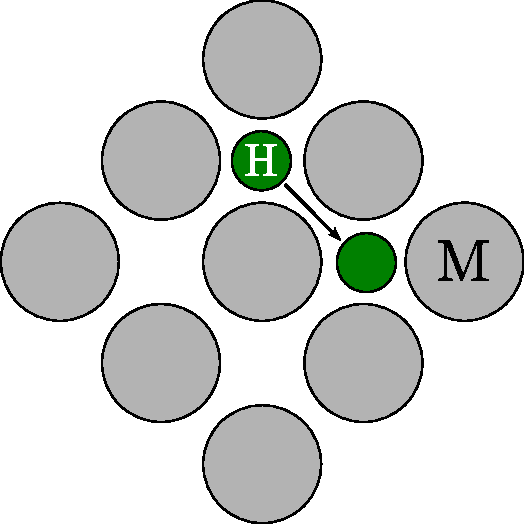
\includegraphics[width=2.5cm]{Images/CL.pdf}}; 
    \end{tikzpicture}
    
    \begin{tikzpicture}[remember picture, overlay]
		\node at (current page.south west) [xshift=10cm, yshift=2.5cm] {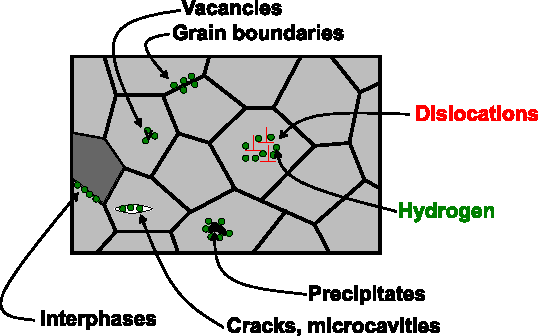
\includegraphics[width=4.5cm]{Images/CT.pdf}}; 
	\end{tikzpicture}
     
	\begin{textblock}{5}(1,14.)
        \textcolor{NewRed}{\footnotesize (Coupling terms)}
    \end{textblock}

\end{frame}

%%%%%%%%%%%%%%%%%%%%%%%%%%%%%%%%%%%%%%%%%%%%%%%%%%%%%%%%%%%

\begin{frame}{Material damage}

    \begin{itemize}
        \item The \textbf{ductile behavior} of the metal is described by the well-known \textbf{GTN model} (\textcolor{darkgray}{Tvergaard \textit{et al.} 1984}):
     \end{itemize}

        $$ \displaystyle \frac{\sigma_{eq}^2}{\sigma_F^2} + 2 q_1 f_* \cosh \left(\frac{q_2}{2} \frac{\sigma_{ii}}{\sigma_F}\right) - 1 -q_1^2 f_*^2 = 0 \quad \textrm{where} \quad f^* = \textrm{function}(f) $$ 

        \vspace{0.15cm}

        $$ \displaystyle \dot{f} = \dot{f}_{nucleation} + \dot{f}_{growth} $$

        \vspace{0.15cm}

        \begin{figure}
            \centering
            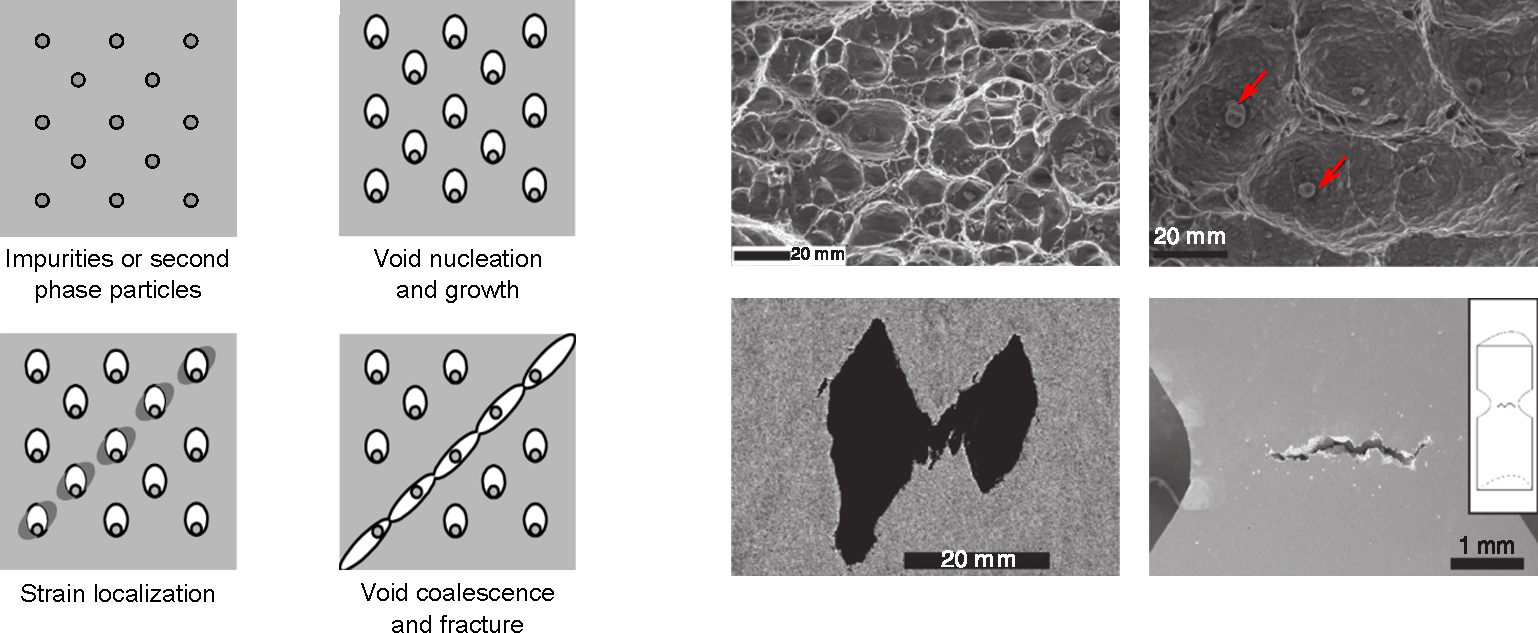
\includegraphics[width=0.9\textwidth]{Images/damage_evolution.pdf}
        \end{figure}
        
\end{frame}

%%%%%%%%%%%%%%%%%%%%%%%%%%%%%%%%%%%%%%%%%%%%%%%%%%%%%%%%%%%

\begin{frame}{Hydrogen embrittlement}

    \begin{itemize}

        \item \textbf{Void growth}: Unchanged due to mass conservation
        
        \begin{equation*}
            \dot{f}_g = (1-f_g) \textrm{trace}(\dot{\varepsilon}_p)
        \end{equation*}  

        \vspace{0.2cm} 
        
        \item\textbf{Void nucleation}: Proposed dependance on hydrogen concentration
        
        \begin{equation*}
            \dot{f}_n = A_n (\kappa) \dot{\kappa} + \textcolor{NewRed}{B_n (C)} \dot{\kappa}
        \end{equation*}

    \end{itemize}
    
    \hspace{1.5cm} 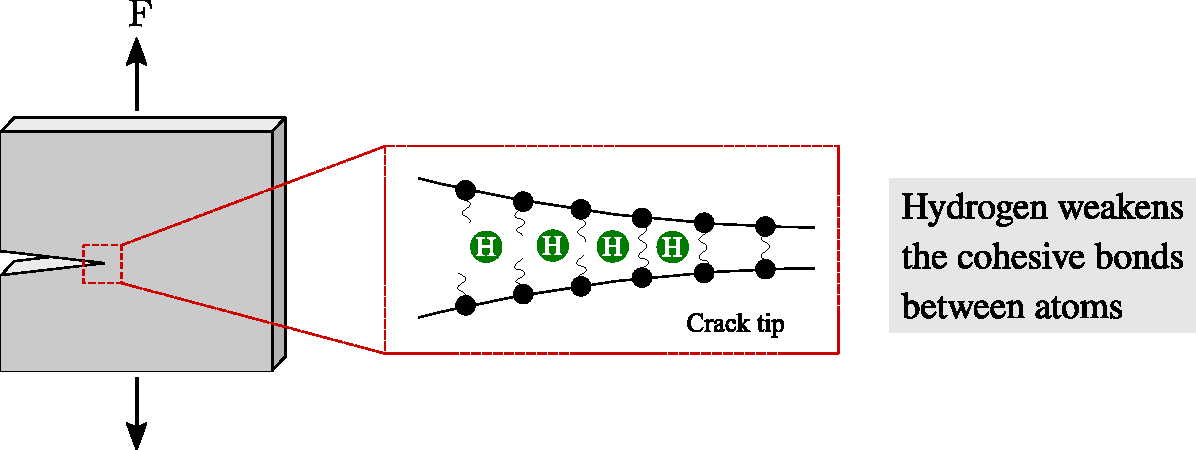
\includegraphics[width=0.75\textwidth]{Images/HEDE3.pdf}

    \begin{textblock}{10}(5,13.5)
        \textcolor{NewRed}{$B_n (C)$}: Damage nucleation due to hydrogen \\ \textbf{HEDE} (Hydrogen Enhanced Decohesion)
    \end{textblock}
    
    \begin{textblock}{5}(13.,7.5)
        \textcolor{NewRed}{\footnotesize (Coupling terms)}
    \end{textblock}

\end{frame}

%%%%%%%%%%%%%%%%%%%%%%%%%%%%%%%%%%%%%%%%%%%%%%%%%%%%%%%%%%%

\section{Finite element formulation}

\begin{frame}{Outline}
	\tableofcontents[ 
    currentsubsection, 
    hideothersubsections, 
    sectionstyle=show/shaded, 
    subsectionstyle=show/shaded, 
    ] 
\end{frame}

%%%%%%%%%%%%%%%%%%%%%%%%%%%%%%%%%%%%%%%%%%%%%%%%%%%%%%%%%%%

\begin{frame}{Mixed formulation}

    \begin{itemize}
        \item Fully implicit finite strain framework
        \vspace{0.1cm}
        \item Based on a mixed formulation: $\underline{u}, p, \theta$ (\textcolor{darkgray}{Zhang \textit{et al.} 2017}) and $C_L$ 
        \vspace{0.1cm}
        \item Quadratic elements with reduced integration
        \vspace{0.1cm}
        \item \textbf{Aim:} better pressure fields by avoiding volumetric locking
    \end{itemize}

    \begin{block}{\textbf{Advantage}}
        $\textcolor{NewRed}{\nabla p}$ can be directly computed from nodal values
        \begin{equation*}
            J = {-D_L \nabla C_L} + {{\frac{D_L C_L V_H}{RT} \textcolor{NewRed}{\nabla p}}}
        \end{equation*} 
    \end{block}
    
    \vspace{0.1cm}
    
    \begin{figure}
        \centering
        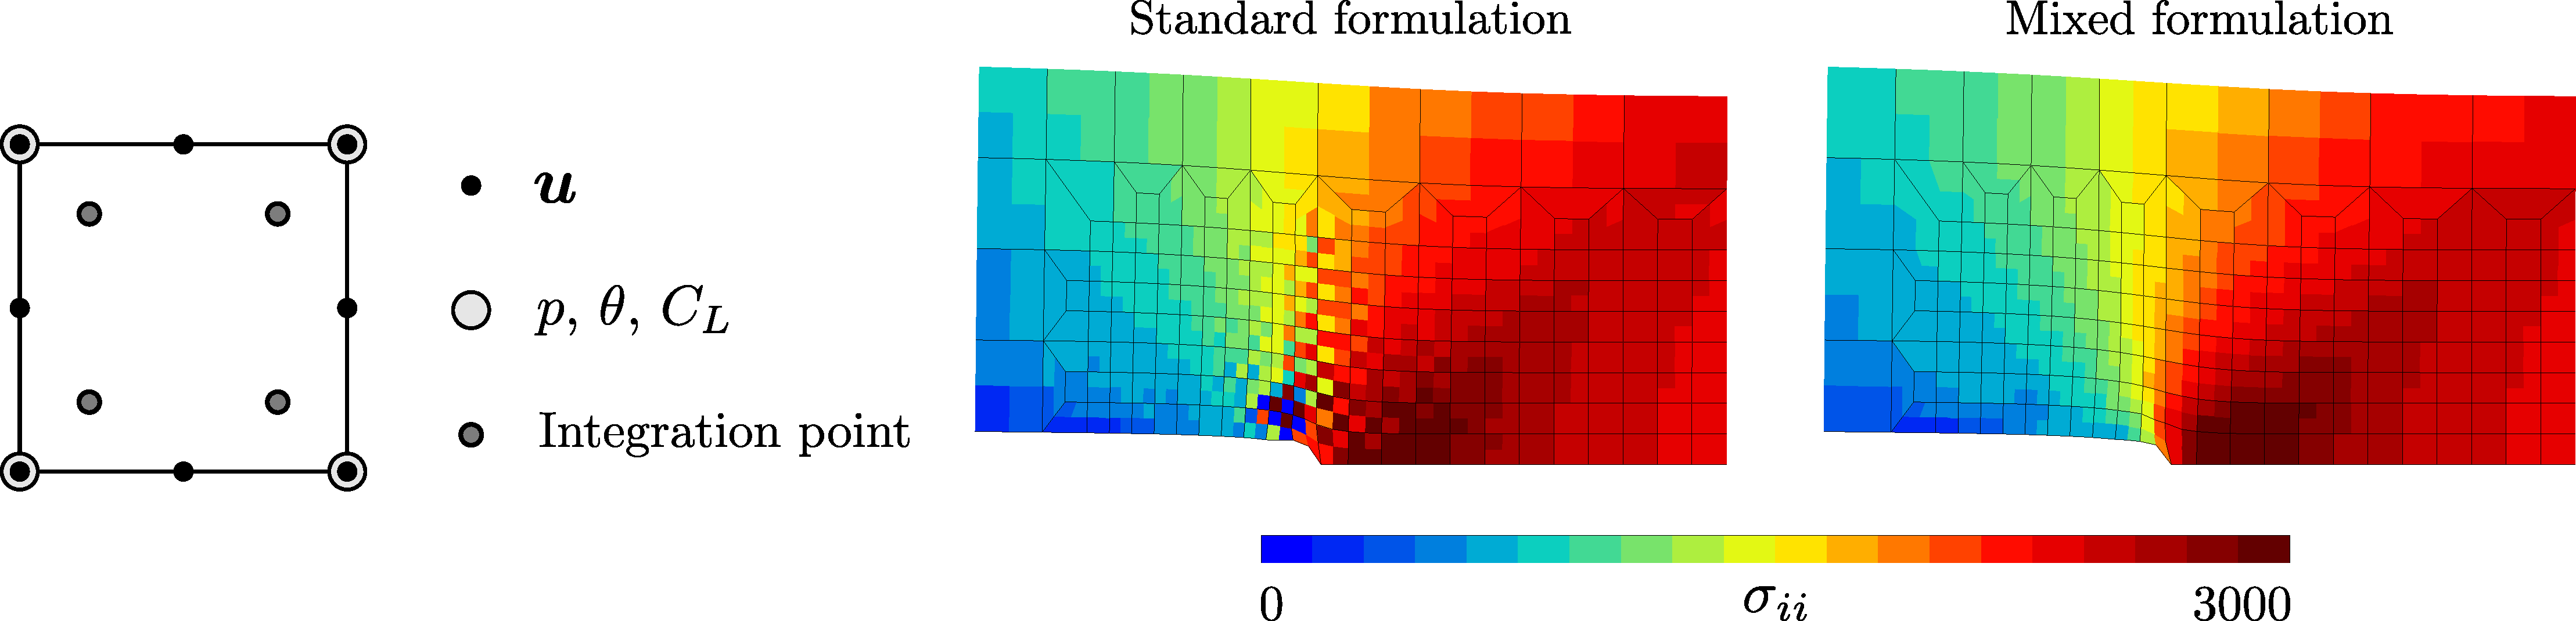
\includegraphics[width=1.\textwidth]{Images/volumetric_locking.pdf}
    \end{figure}

    \begin{tikzpicture}[remember picture, overlay]
        \node at (current page.south west) [xshift=11.5cm, yshift=7.5cm] {
\includegraphics[width=2cm]{Images/Zset.jpg}}; 
    \end{tikzpicture}

\end{frame}

%%%%%%%%%%%%%%%%%%%%%%%%%%%%%%%%%%%%%%%%%%%%%%%%%%%%%%%%%%%

\begin{frame}{$\boldsymbol{B}$-bar formulation}
    
	\begin{itemize}
		\item The use of \textbf{quadratic elements} with additional dofs can be very \\ \textbf{time consuming}
		\vspace{0.25cm}
		\item $\boldsymbol{B}$-bar (or $\boldsymbol{\bar{B}}$) formulation (\textcolor{darkgray}{Hughes, 1980}): 
		\vspace{0.25cm}
		\begin{itemize}
			\item Linear elements with full integration
			\vspace{0.25cm}
			\item Solves volumetric locking by modifying the strain-displacement matrix: \\
			$$\boldsymbol{\bar{B}} = \boldsymbol{B}_d + \boldsymbol{\bar{B}}_h$$
			\vspace{0.05cm}
			\item To avoid extrapolating $p$ to the nodes for $\nabla p$ computation, it is considered as a dof
%			\vspace{0.05cm}
%			$$ \min(P_{pg} - N \cdot P_n)^2 $$
		\end{itemize}
	\end{itemize}	
	
	\vspace{0.25cm}	
	
	\begin{figure}
        \centering
        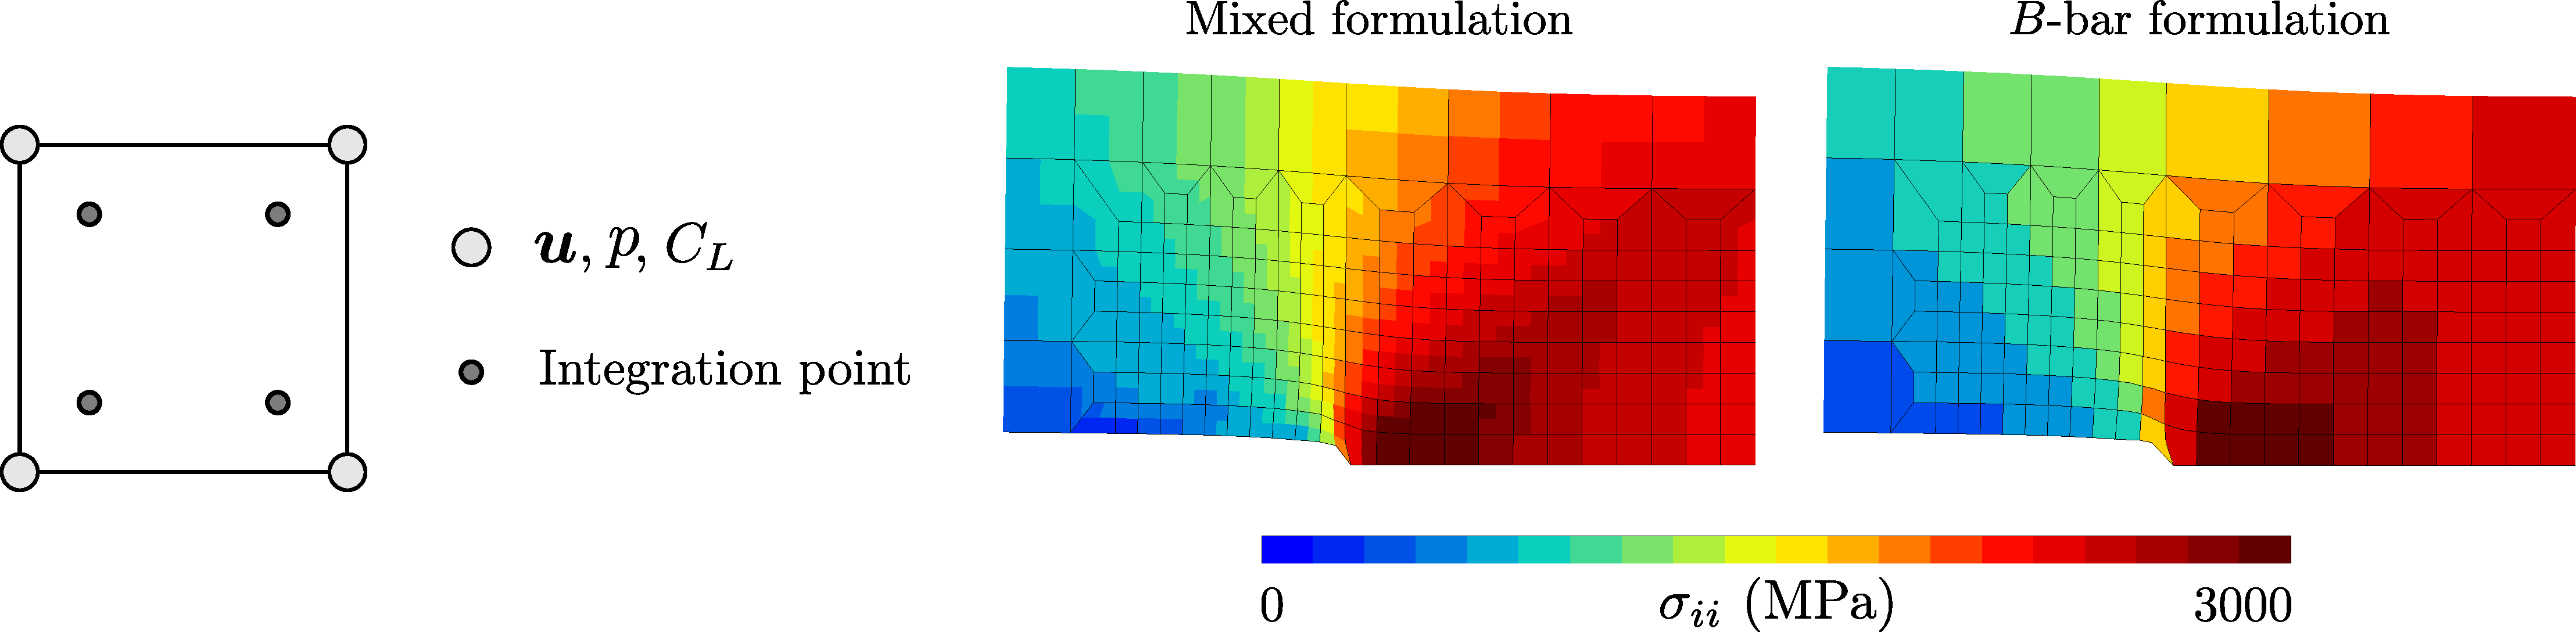
\includegraphics[width=1.\textwidth]{Images/comp_nlgeom-3f_B-bar.pdf}
    \end{figure}  
    
    \begin{tikzpicture}[remember picture, overlay]
        \node at (current page.south west) [xshift=11.5cm, yshift=7.5cm] {
\includegraphics[width=2cm]{Images/Zset.jpg}}; 
    \end{tikzpicture}  
    
\end{frame}

%%%%%%%%%%%%%%%%%%%%%%%%%%%%%%%%%%%%%%%%%%%%%%%%%%%%%%%%%%%

\begin{frame}{$\boldsymbol{B}$-bar formulation}

	\begin{itemize}
		\item Test on a Disk Compact Tension (DCT) specimen with 5200 elements:
		\vspace{0.25cm}
		
		\begin{itemize}
			\item \textbf{Mixed formulation}: 103,762 dofs, 1h 40 minutes to complete
			\vspace{0.25cm}
			\item $\boldsymbol{B}$\textbf{-bar formulation}: 33,974 dofs, 18 minutes to complete
		\end{itemize}
		\vspace{0.25cm}
		\item Slightly higher force for the $\boldsymbol{B}$-bar formulation $\rightarrow$ Linear elements are inherently stiffer since they have less nodes  
	\end{itemize}
	
\begin{columns}
	\begin{column}{0.5\textwidth}
		\begin{figure}
        \centering
        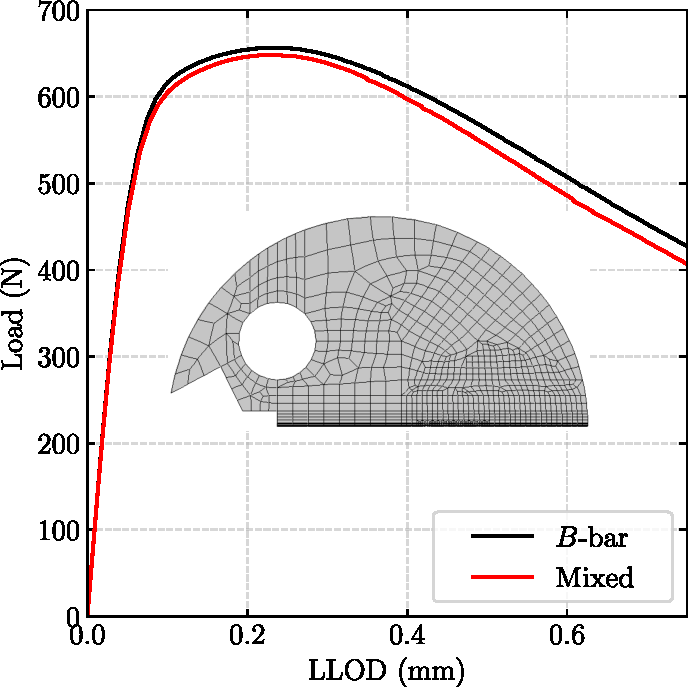
\includegraphics[width=0.7\textwidth]{Images/Load_LLOD_Bbar.pdf}
    \end{figure} 
	\end{column}
	
	\begin{column}{0.5\textwidth}
		\begin{figure}
        \centering
        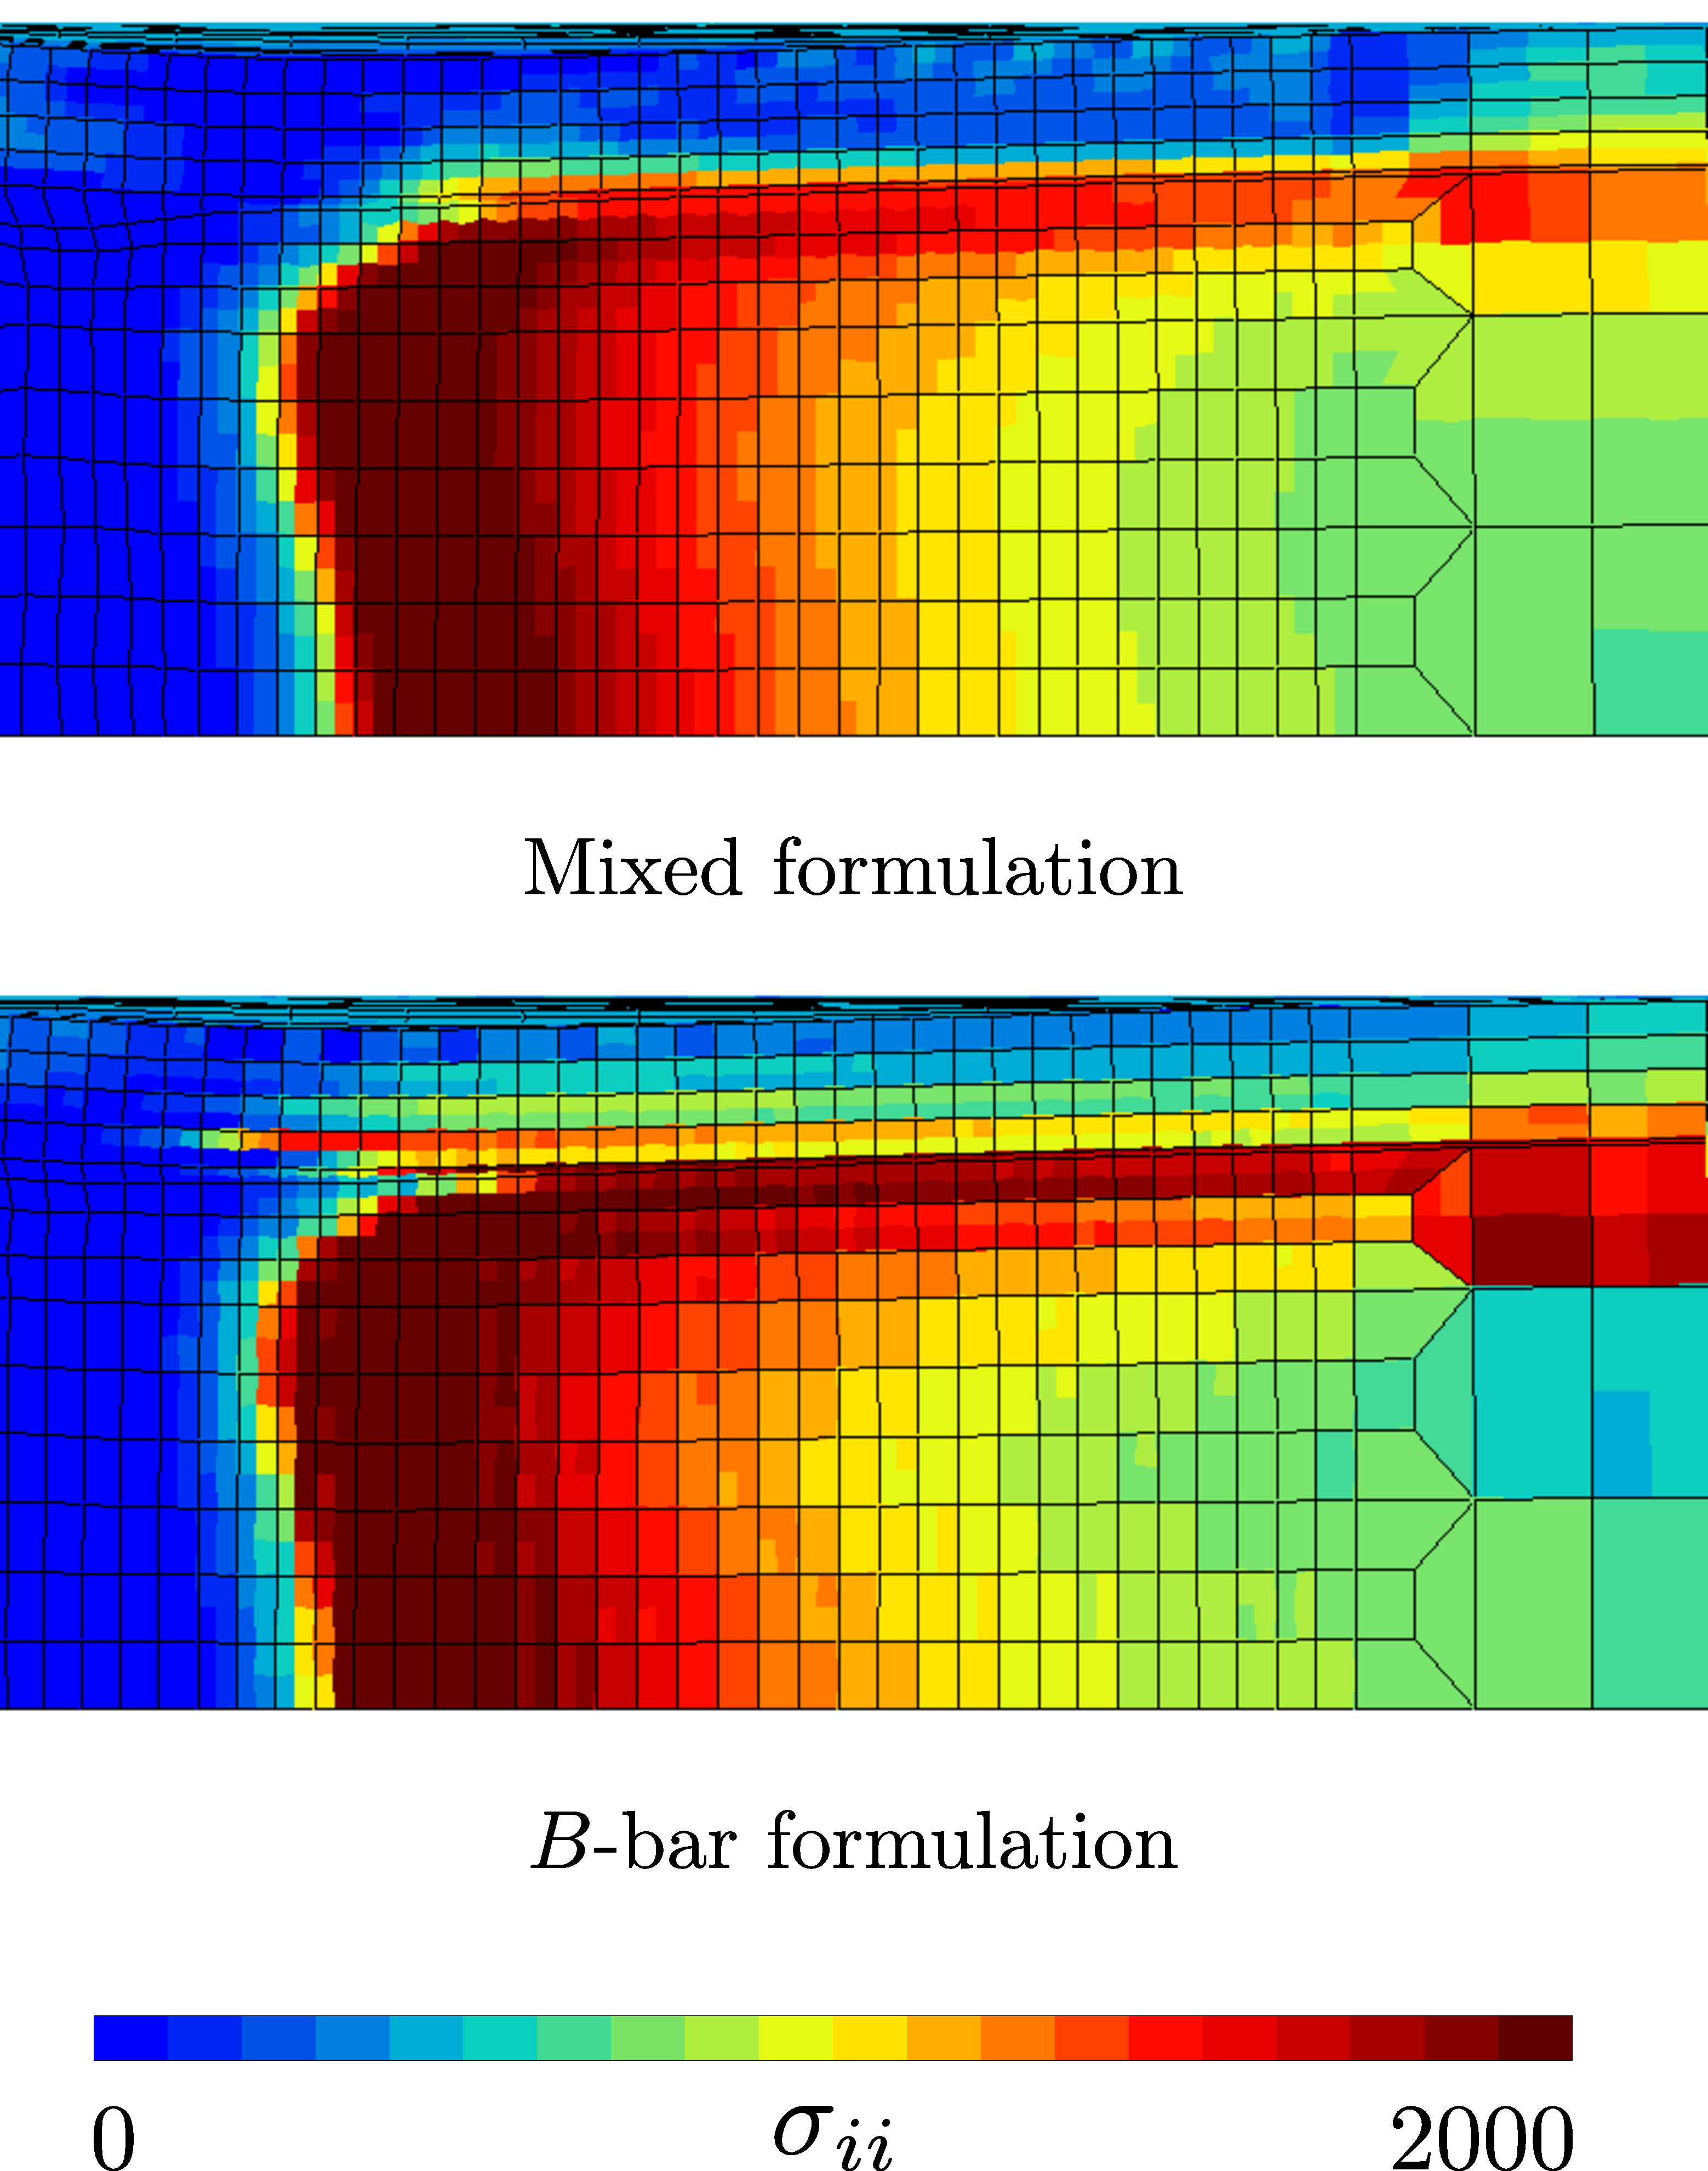
\includegraphics[width=0.6\textwidth]{Images/pressure_Bbar.pdf}
    \end{figure} 
	\end{column}
\end{columns}

\end{frame}

%%%%%%%%%%%%%%%%%%%%%%%%%%%%%%%%%%%%%%%%%%%%%%%%%%%%%%%%%%%

\begin{frame}{Nonlocal damage model}

\begin{itemize}
	\item Damage models such as the GTN model are known to induce \textbf{spurious mesh dependency} (element size, type and orientation)
	\vspace{0.25cm}
	\item To solve this problem, it is proposed to use a \textbf{nonlocal damage model} based on the \textbf{implicit gradient} by \textcolor{darkgray}{Peerlings \textit{et al.}, 1996}
\end{itemize}

	\vspace{0.25cm}

	\begin{figure}
        \centering
        \includegraphics[width=0.9\textwidth]{Images/mesh_dependency.pdf}
    \end{figure} 
    
    \begin{textblock}{5}(7.2,14.25)
        \textcolor{darkgray}{\footnotesize (Besson, 2021)}
    \end{textblock}

\end{frame}

%%%%%%%%%%%%%%%%%%%%%%%%%%%%%%%%%%%%%%%%%%%%%%%%%%%%%%%%%%%

\begin{frame}{Nonlocal damage model}

	\begin{itemize}
		\item Two variables are used (two associated internal lengths: $\bar{\omega}$ and $\bar{\kappa}$):
		
		\vspace{0.15cm}
		
        \begin{itemize}

            \item $ \displaystyle \textbf{Plastic volume variation:} \hspace{0.7cm} \textcolor{blue}{\bar{\omega}} - \ell_{\omega}^2 \Delta \textcolor{blue}{\bar{\omega}} = \omega \hspace{0.3cm} \textrm{where} \hspace{0.3cm} \omega = \textrm{trace}(\dot{\underline{\varepsilon}}_p)$
            
            \vspace{0.3cm}
            
            \item $ \displaystyle \textbf{Accumulated plastic strain:} \hspace{0.3cm} \textcolor{red}{\bar{\kappa}} - \ell_{\kappa}^2 \Delta \textcolor{red}{\bar{\kappa}} = \kappa \hspace{3.6cm}$

        \end{itemize}
        
        \vspace{0.3cm}
        
		\item The modified evolution laws for the damage variables are now:
		
        \vspace{0.3cm}
        
        \begin{itemize}
        
            \item \textbf{Void growth:} \hspace{0.7cm} $ \displaystyle \dot{f_g} = (1-f_g) \textcolor{blue}{\dot{\bar{\omega}}} $
            
            \vspace{0.3cm}
            
            \item \textbf{Void nucleation:} \hspace{0.2cm} $ \displaystyle \dot{f_n} = A_n \textcolor{red}{\dot{\bar{\kappa}}} + B_n(C) \textcolor{red}{\dot{\bar{\kappa}}}$
            
        \end{itemize}        
               
	\end{itemize}
	
	\vspace{2.65cm}
	
	\begin{tikzpicture}[remember picture, overlay]
    	\node at (current page.south west) [xshift=4.5cm, yshift=2.1cm] {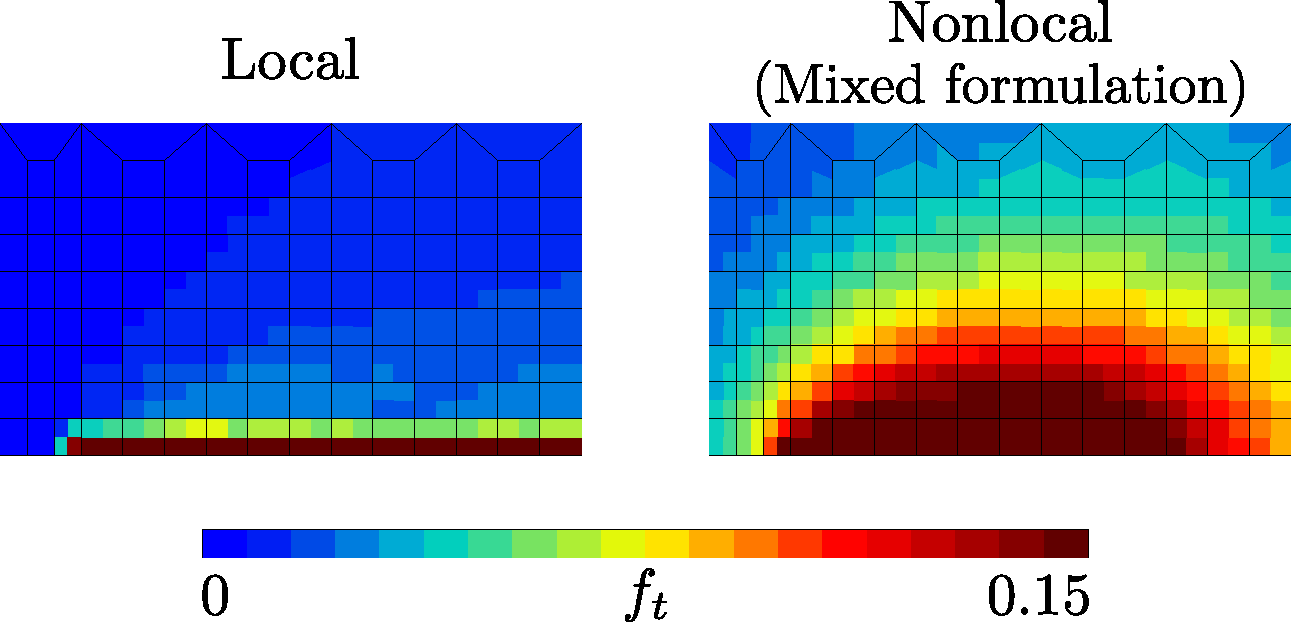
\includegraphics[width=6cm]{Images/comp_ft.pdf}}; 
    \end{tikzpicture}
    
    \begin{tikzpicture}[remember picture, overlay]
    	\node at (current page.south west) [xshift=10.5cm, yshift=3.1cm] {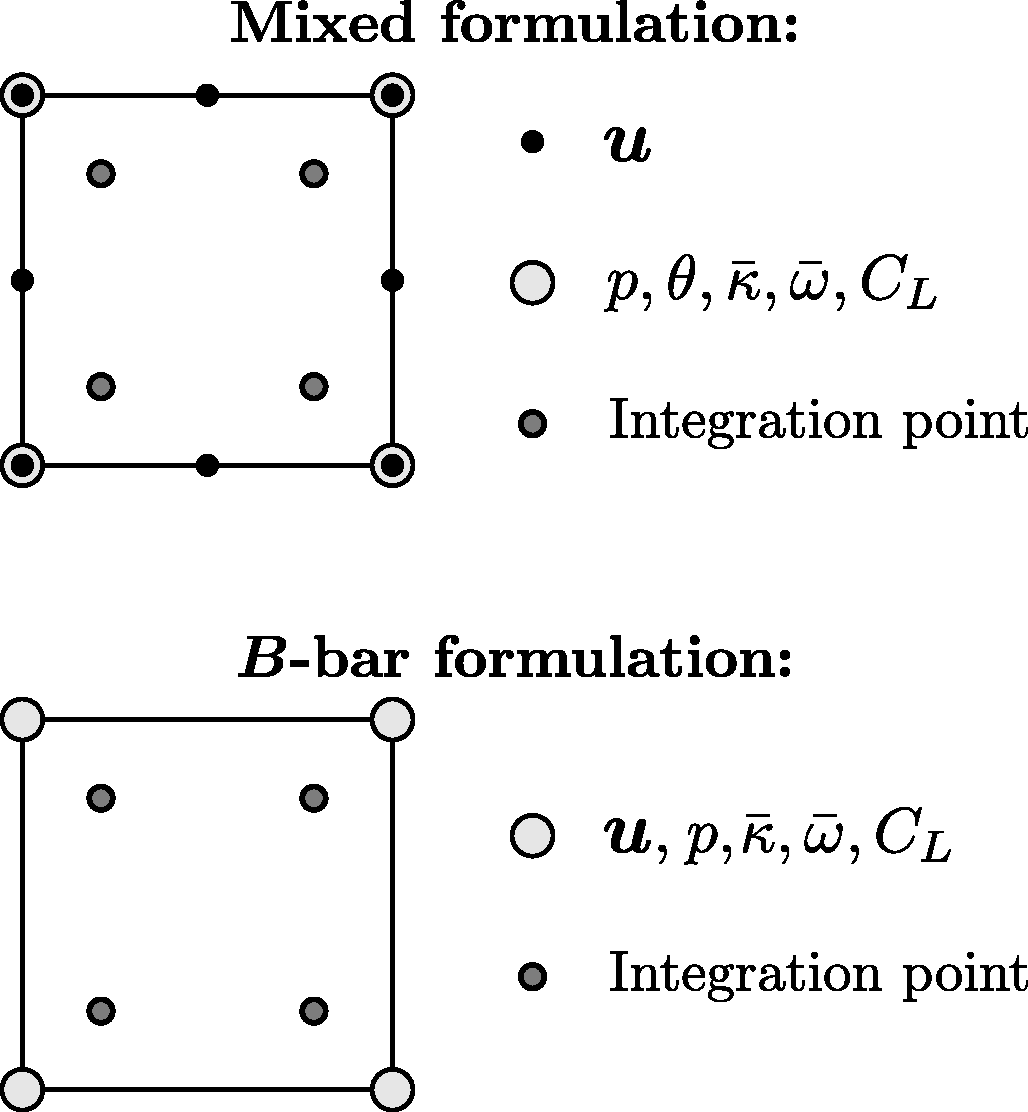
\includegraphics[width=4cm]{Images/elements.pdf}}; 
    \end{tikzpicture}

\end{frame}

%%%%%%%%%%%%%%%%%%%%%%%%%%%%%%%%%%%%%%%%%%%%%%%%%%%%%%%%%%%

\section{Numerical simulations}

\subsection{Pressurized disks tests}

\begin{frame}{Outline}
	\tableofcontents[ 
    currentsubsection, 
    hideothersubsections, 
    sectionstyle=show/shaded, 
    subsectionstyle=show/shaded, 
    ] 
\end{frame}

%%%%%%%%%%%%%%%%%%%%%%%%%%%%%%%%%%%%%%%%%%%%%%%%%%%%%%%%%%%

\begin{frame}{Context}

	\begin{itemize}
		\item \textbf{ISO 11114-4 standard:} uses pressurized disk tests for selecting metallic materials resistant to hydrogen embrittlement
		\vspace{0.15cm}
		\item Disk often fails in the clamping zone
		\vspace{0.15cm}
		\item \textbf{\textcolor{MINESBlue}{First step:}} redesigning the disk geometry to control failure location
	\end{itemize}
	
	\vspace{5cm}
	
	\begin{tikzpicture}[remember picture, overlay]
    	\node at (current page.south west) [xshift=3cm, yshift=3.5cm] {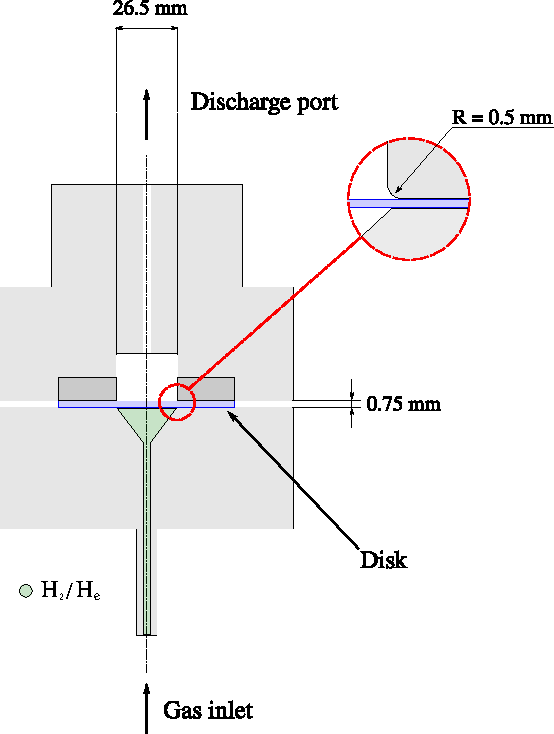
\includegraphics[width=4cm]{Images/machine_DPT.pdf}}; 
    \end{tikzpicture}
    
    \begin{tikzpicture}[remember picture, overlay]
    	\node at (current page.south west) [xshift=6.75cm, yshift=5.5cm] {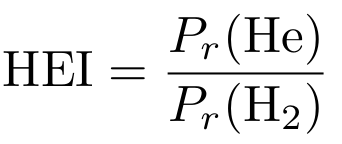
\includegraphics[width=2.cm]{Images/HEI.png}}; 
    \end{tikzpicture}
    
    \begin{tikzpicture}[remember picture, overlay]
    	\node at (current page.south west) [xshift=6.35cm, yshift=3cm] {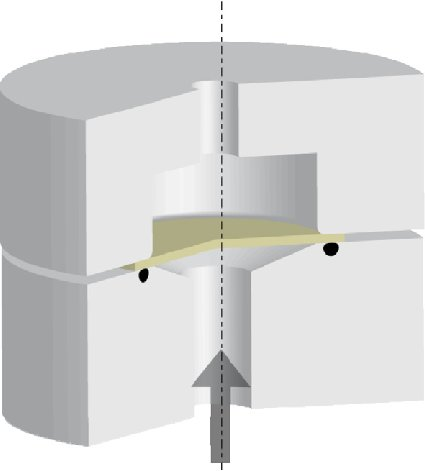
\includegraphics[width=2.75cm]{Images/machine_DPT_2.jpg}}; 
    \end{tikzpicture}
    
    \begin{tikzpicture}[remember picture, overlay]
    	\node at (current page.south west) [xshift=10.5cm, yshift=5cm] {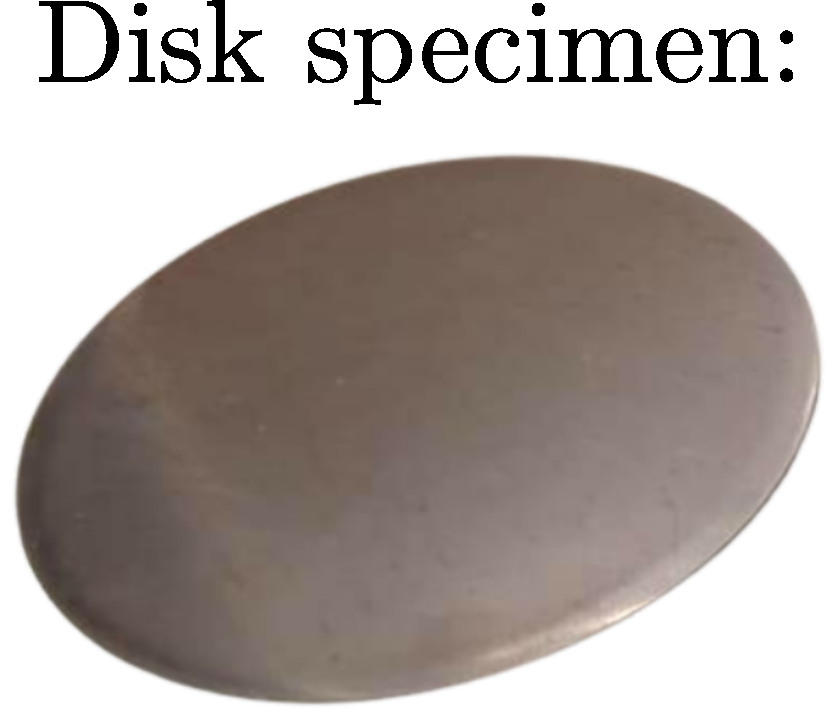
\includegraphics[width=2.cm]{Images/std_disk.pdf}}; 
    \end{tikzpicture}
    
    \begin{tikzpicture}[remember picture, overlay]
    	\node at (current page.south west) [xshift=10.5cm, yshift=2.5cm] {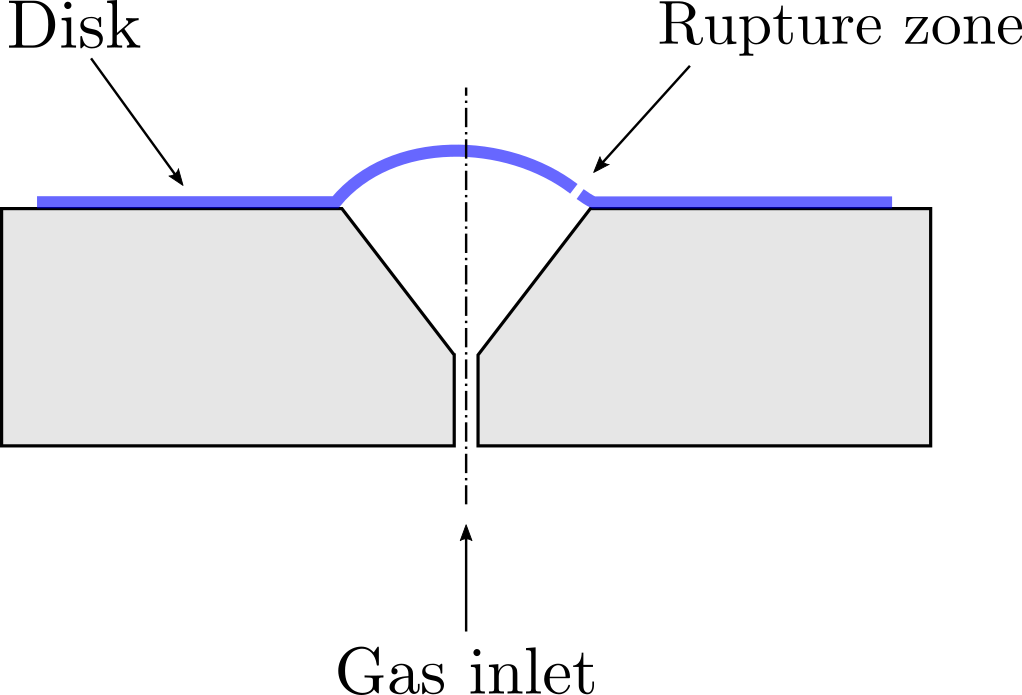
\includegraphics[width=4cm]{Images/rupture_disk.png}}; 
    \end{tikzpicture}
	
\end{frame}

%%%%%%%%%%%%%%%%%%%%%%%%%%%%%%%%%%%%%%%%%%%%%%%%%%%%%%%%%%%

\begin{frame}{Redesign of the disk geometry}

\begin{itemize}
	\item New proposed geometries:
	\vspace{0.15cm}
	\begin{itemize}
		\item No need to modify the test setup
		\vspace{0.15cm}
		\item Keep the same minimum thickness of the standard (0.75 mm)
		\vspace{0.15cm}
	\end{itemize}
	\item Optimization with respect to $\ell$, $R$ and $R^\prime$ with FE simulations considering an elasto-plastic behavior
\end{itemize}

\begin{figure}
	\centering
	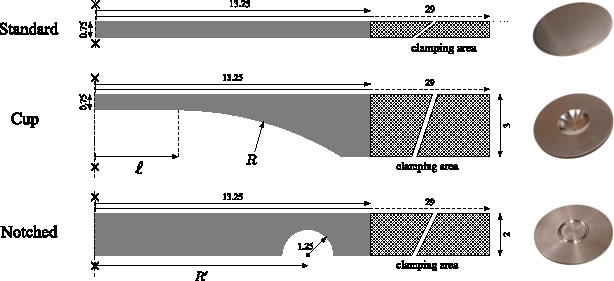
\includegraphics[width=0.9\textwidth]{Images/disks.pdf}
\end{figure}

\end{frame}

%%%%%%%%%%%%%%%%%%%%%%%%%%%%%%%%%%%%%%%%%%%%%%%%%%%%%%%%%%%

\begin{frame}{Redesign of the disk geometry}

\begin{itemize}
	\item The location of the maximum accumulated plastic strain ($\kappa$) corresponds to the failure location
\end{itemize}

\vspace{0.5cm}

\begin{figure}
	\centering
	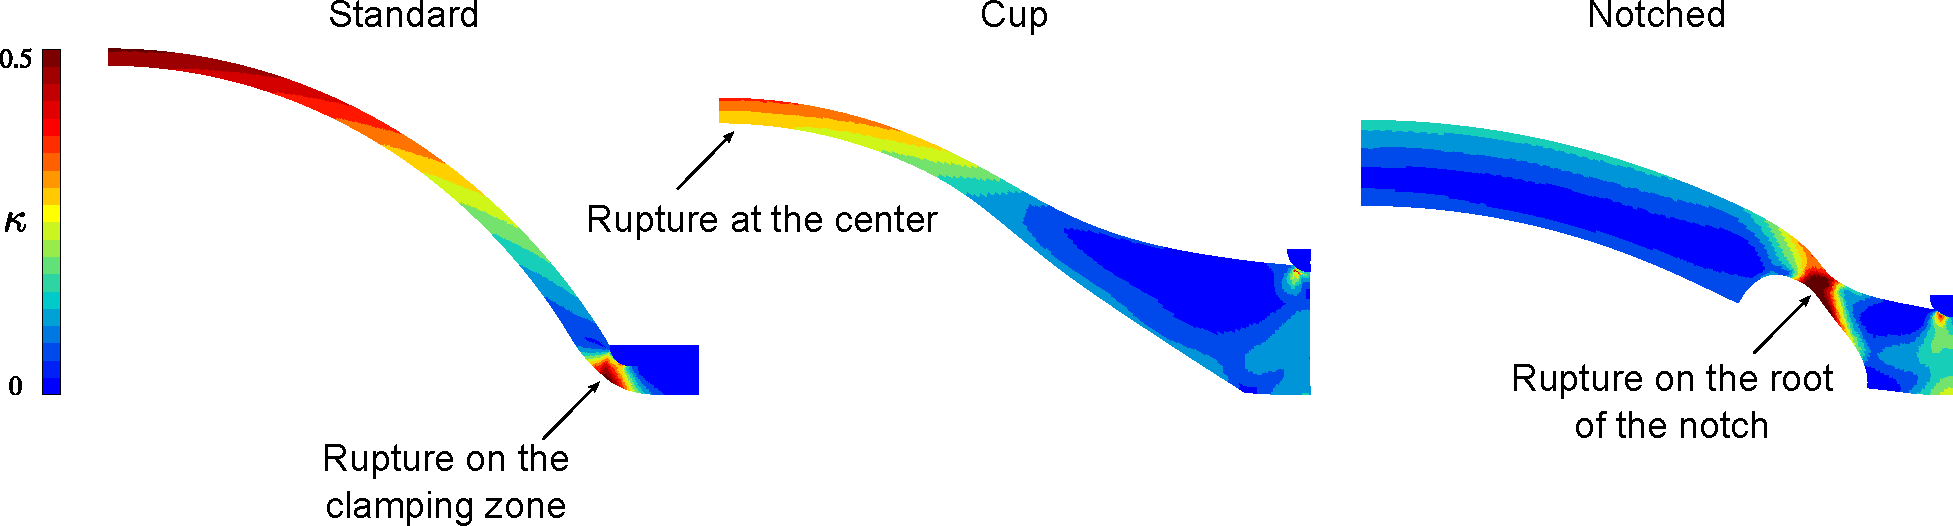
\includegraphics[width=0.95\textwidth]{Images/disks_rupture.pdf}
\end{figure}

\end{frame}

%%%%%%%%%%%%%%%%%%%%%%%%%%%%%%%%%%%%%%%%%%%%%%%%%%%%%%%%%%%

\begin{frame}{Materials}

\begin{columns}
\begin{column}{0.65\textwidth}

\begin{itemize}
	\item \textbf{X52 vintage steel:}
	\vspace{0.3cm}
	\begin{itemize}
		\item Yield strength: 400 MPa
		\vspace{0.3cm}
		\item Different elongation at rupture in T and L directions
	\end{itemize}
	
	\vspace{0.35cm}
	
	\item \textbf{E355 mod. steel:}
	
	\vspace{0.3cm}
	
	\begin{itemize}
		\item Yield strength: 330 MPa
		\vspace{0.3cm}
		\item Higher elongation at rupture and lower Ultimate Tensile Strength in relation with the vintage material
		\vspace{0.cm}
		\item Similar elongation at rupture in both directions
	\end{itemize}
	
	\vspace{0.35cm}	
	
	\item Elasto(visco)-plastic model coefficients' identified through optimization: \\
	
	\begin{figure}
	\centering
	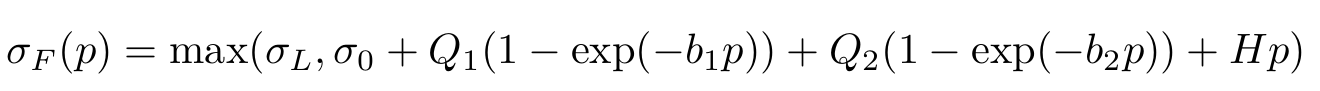
\includegraphics[width=0.98\textwidth]{Images/voce_law.png} \\
\end{figure}

\end{itemize}

\end{column}

\begin{column}{0.35\textwidth}
	
\begin{figure}
	\centering
	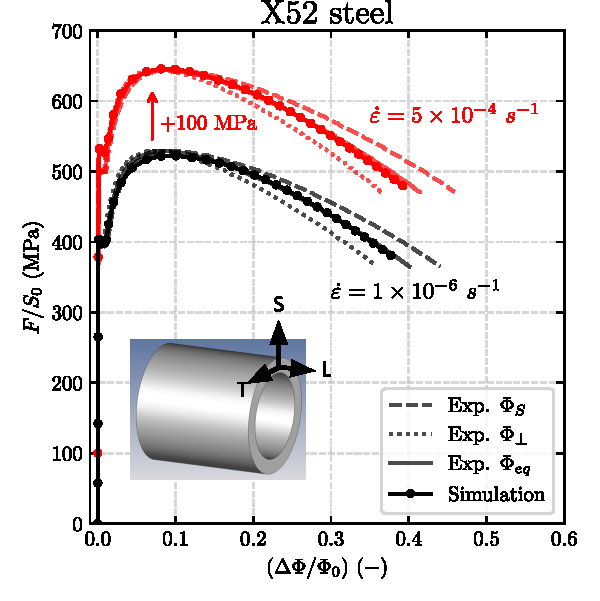
\includegraphics[width=0.95\textwidth]{Images/plot_X52_radial.pdf} \\
	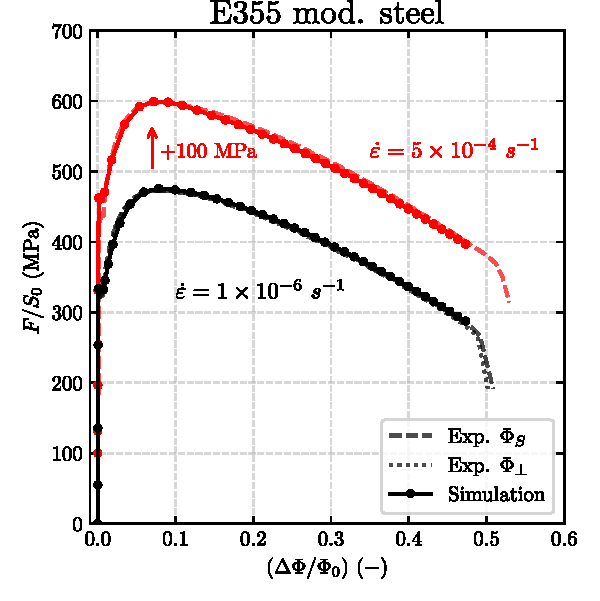
\includegraphics[width=0.95\textwidth]{Images/plot_E355_radial.pdf}
\end{figure}

\end{column}

\end{columns}

\end{frame}

%%%%%%%%%%%%%%%%%%%%%%%%%%%%%%%%%%%%%%%%%%%%%%%%%%%%%%%%%%%

\begin{frame}{Simulation of pressurized disks}

\begin{itemize}
	\item Axisymmetric model, quadratic elements with reduced integration (mixed formulation)
	\vspace{0.15cm}
	\item Hydrogen diffusion parameters taken from the literature
	\vspace{0.15cm}
	\item Since damage is not considered into the numerical model, the simulations were stopped once they reached experimentally observed rupture pressure $(P_r)$
	\vspace{0.15cm} 
	\item Model's boundary conditions:
\end{itemize}

\begin{figure}
	\centering
	\includegraphics[width=0.7\textwidth]{Images/all_BC_std.pdf} \\
\end{figure}

\end{frame}

%%%%%%%%%%%%%%%%%%%%%%%%%%%%%%%%%%%%%%%%%%%%%%%%%%%%%%%%%%%

\begin{frame}{Results under helium}

\begin{itemize}
	\item Successfully modification of fracture location
	\vspace{0.15cm}
	\item Failure is primarily driven by plasticity and occurs \\ under a limit load scenario
\end{itemize}

\vspace{0.15cm}

\begin{figure}
	\centering
	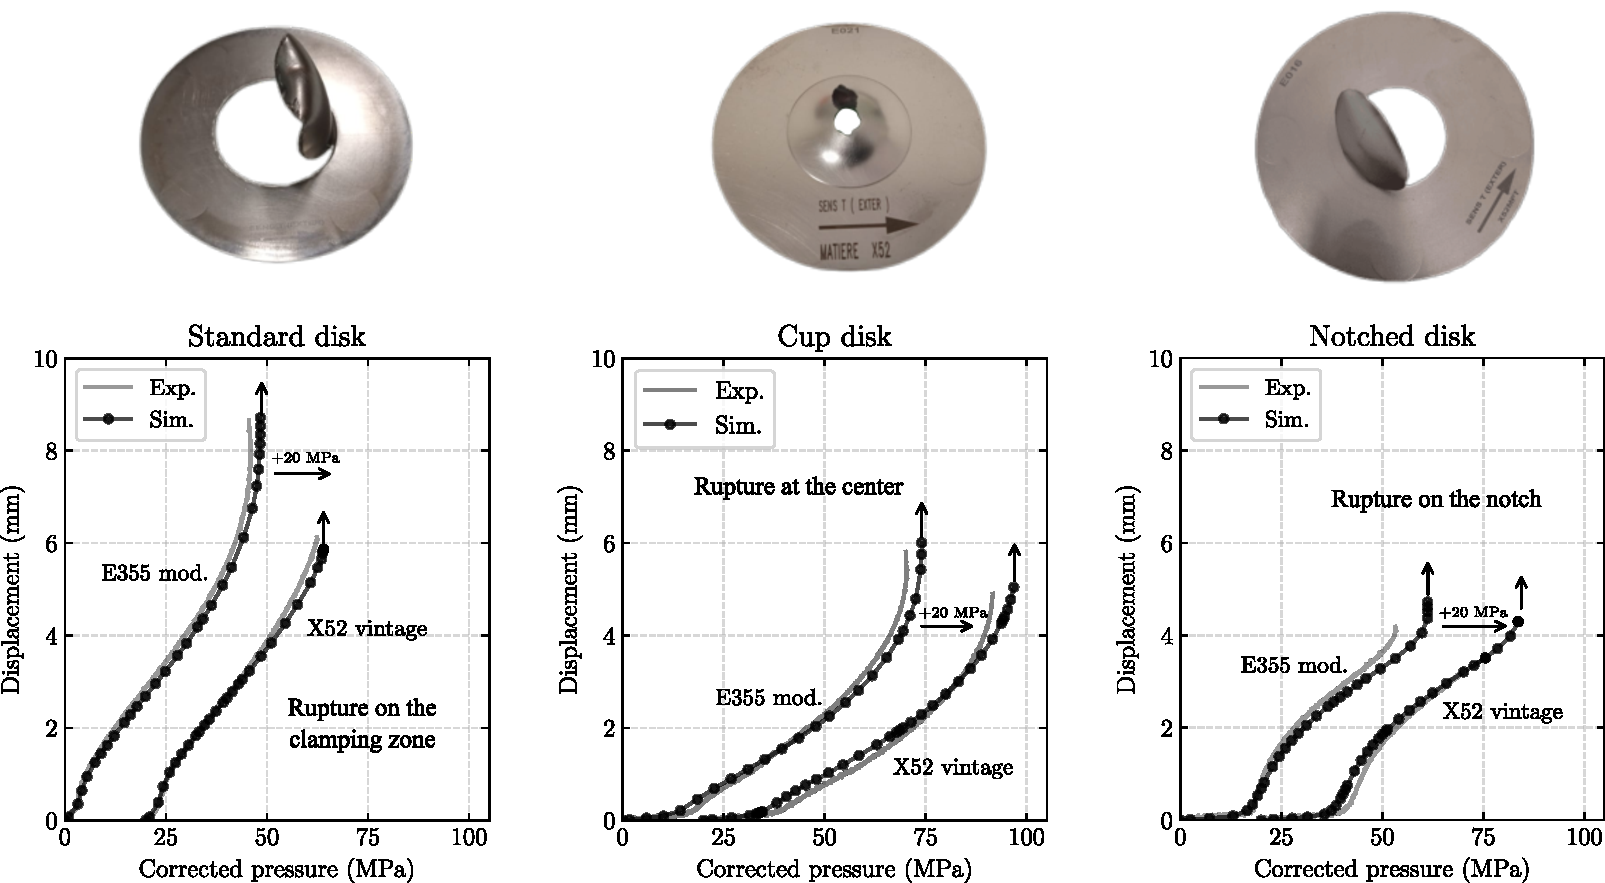
\includegraphics[width=0.85\textwidth]{Images/disks_helium.pdf} \\
\end{figure}

\begin{tikzpicture}[remember picture, overlay]
    	\node at (current page.south west) [xshift=10.2cm, yshift=7.5cm] {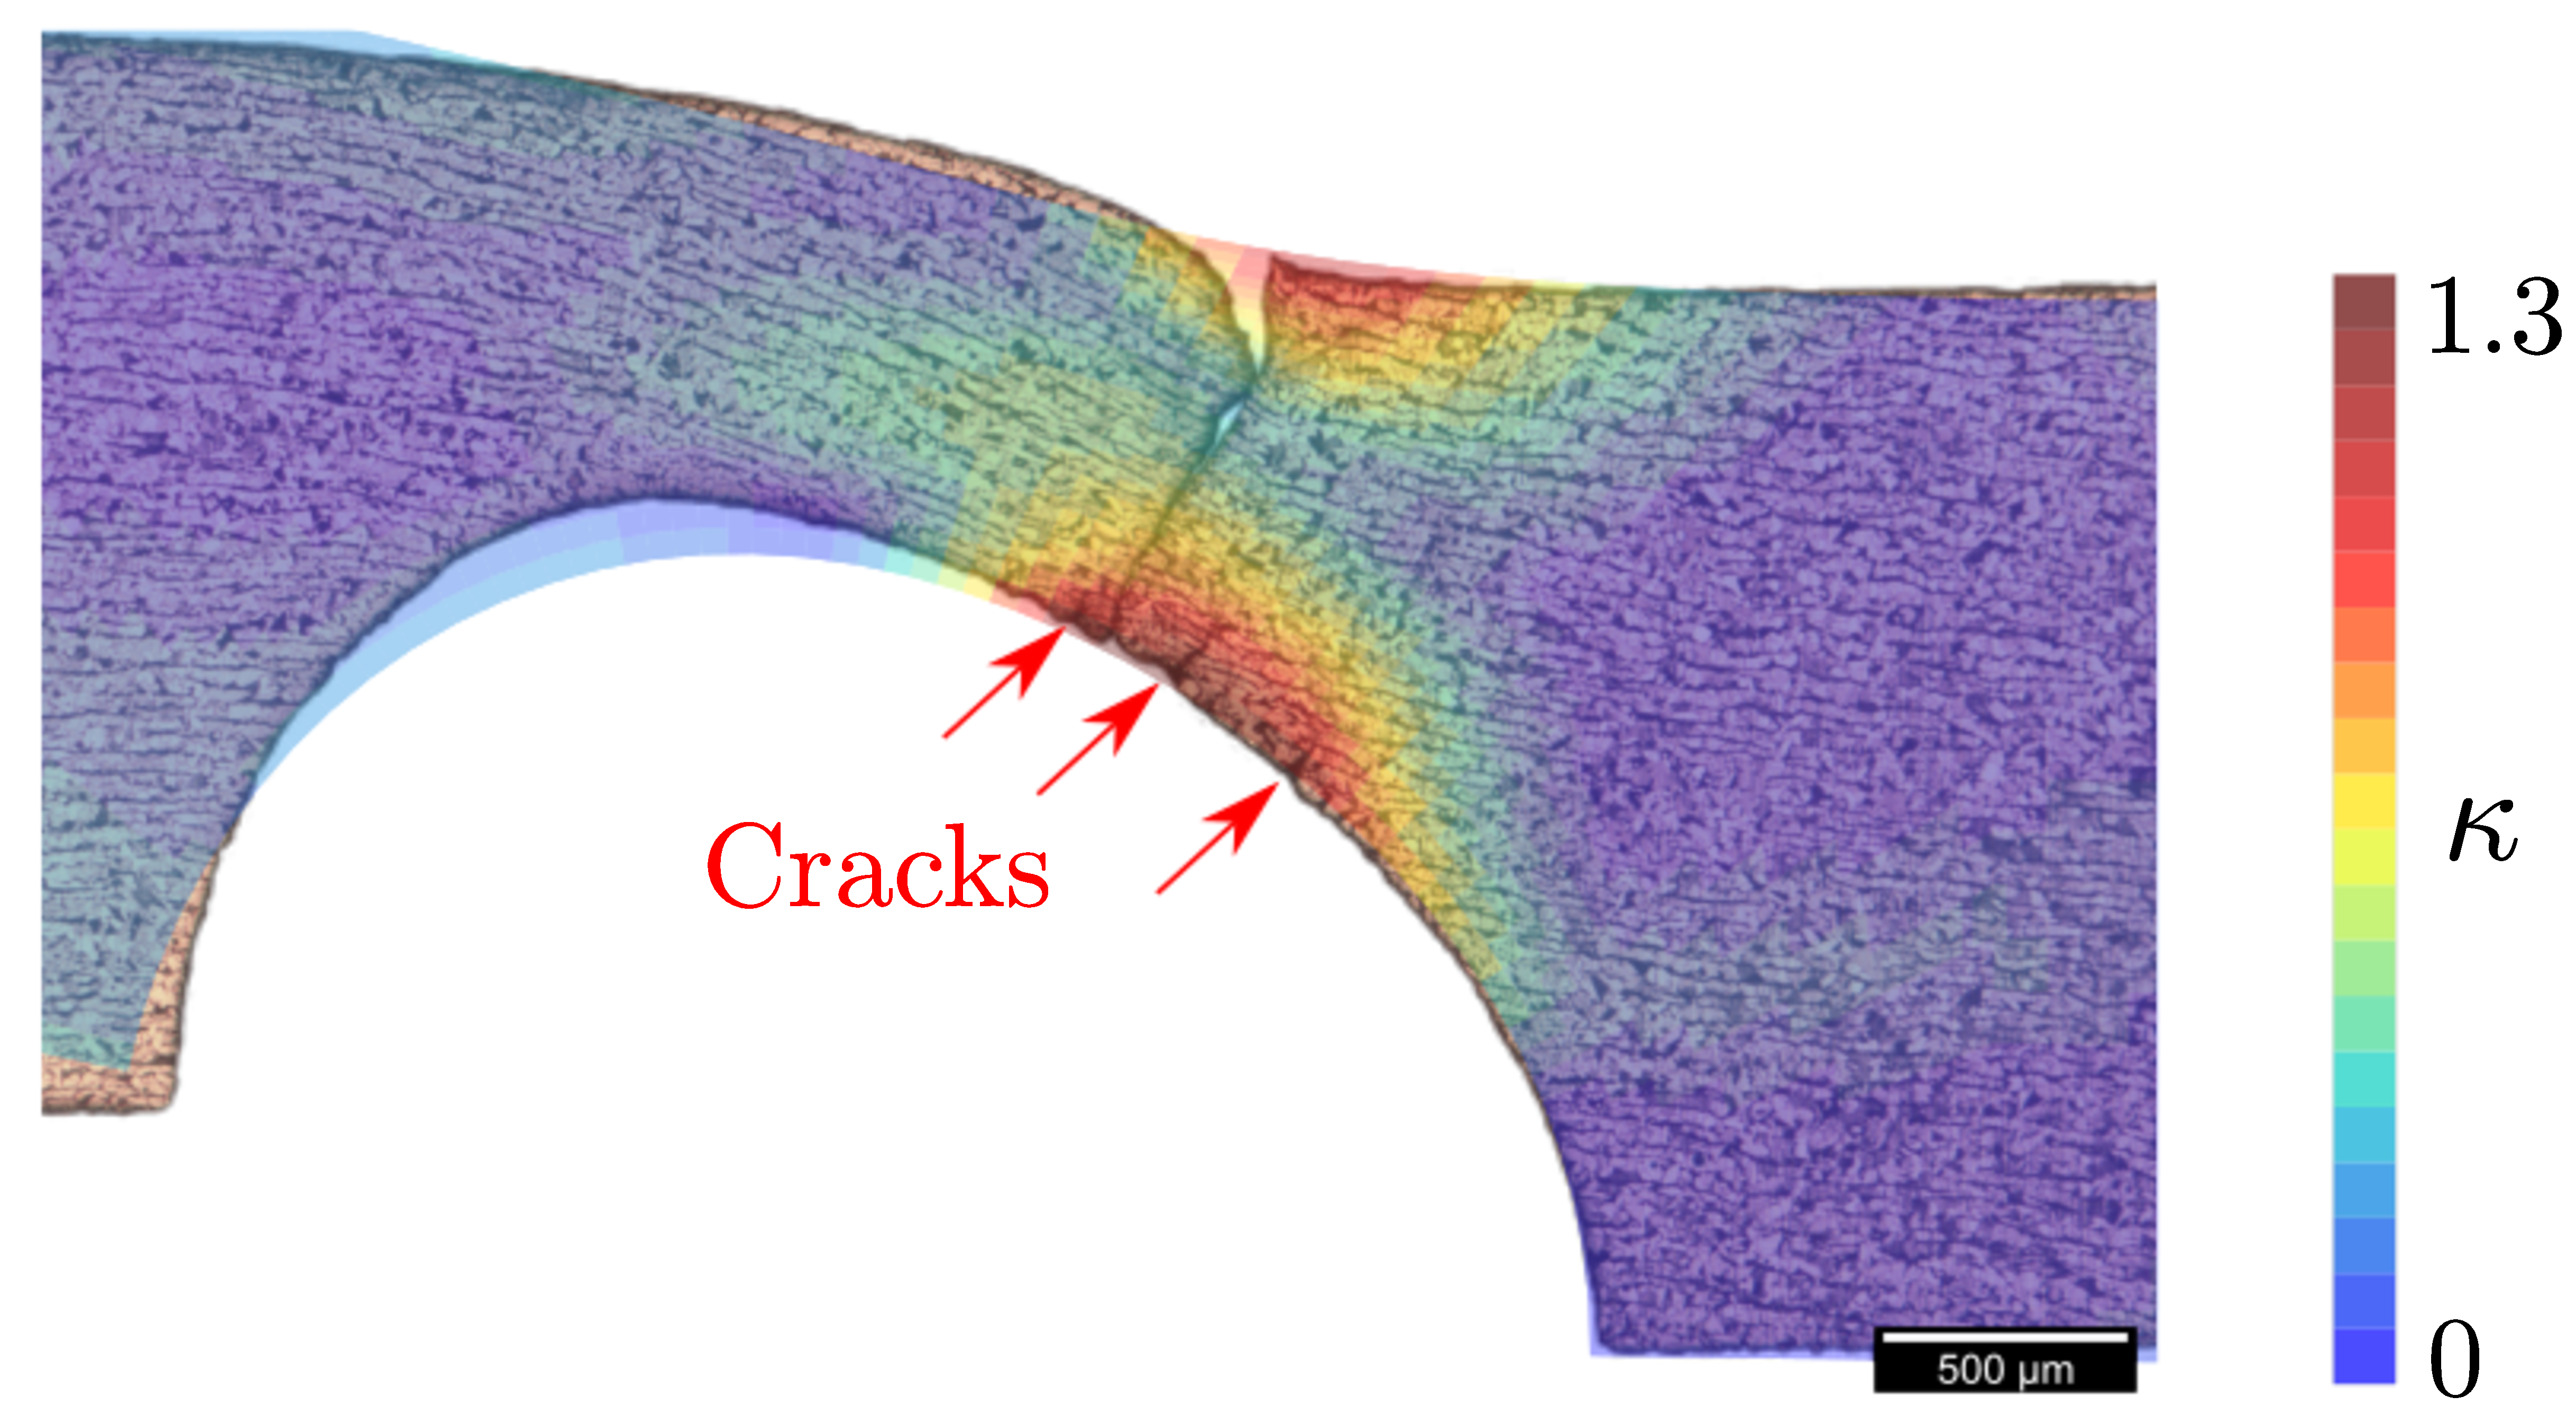
\includegraphics[width=3.75cm]{Images/fracto+simulation.png}}; 
    \end{tikzpicture}
    
    \begin{textblock}{6}(5.75,14.75)
        \textcolor{gray}{\scriptsize (Experimental data: Santana \textit{et al.}, 2024)}
    \end{textblock}

\end{frame}

%%%%%%%%%%%%%%%%%%%%%%%%%%%%%%%%%%%%%%%%%%%%%%%%%%%%%%%%%%%

\begin{frame}{Results under hydrogen (E355 mod. steel)}

\begin{figure}
	\centering
	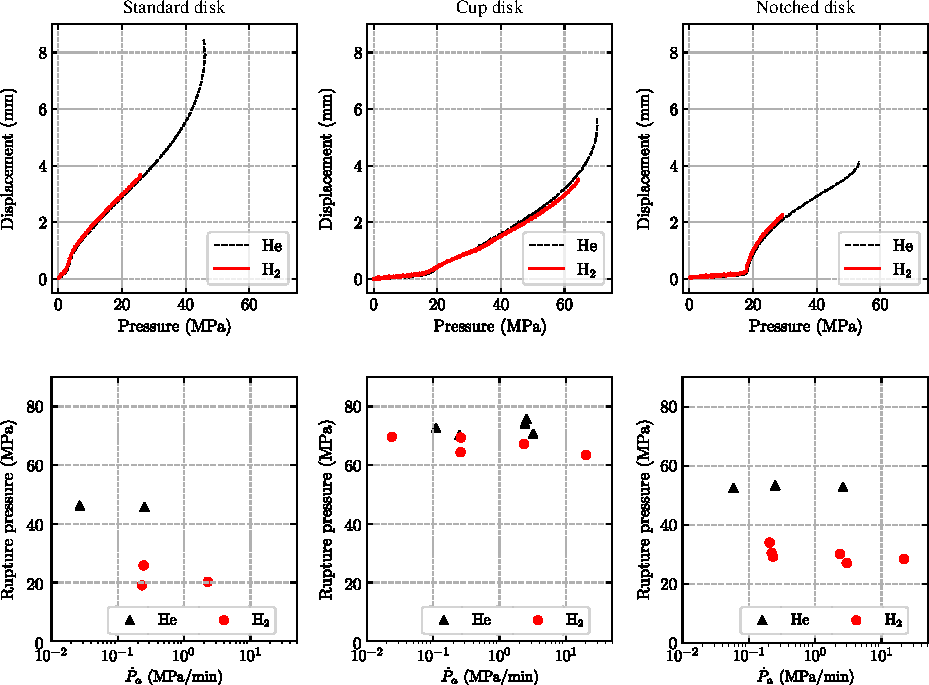
\includegraphics[width=0.85\textwidth]{Images/H2_results_E355.pdf} \\
\end{figure}

    \begin{textblock}{6}(5.75,14.9)
        \textcolor{gray}{\scriptsize (Experimental data: Santana \textit{et al.}, 2024)}
    \end{textblock}

\end{frame}

%%%%%%%%%%%%%%%%%%%%%%%%%%%%%%%%%%%%%%%%%%%%%%%%%%%%%%%%%%%

\begin{frame}{Hydrogen embrittled depth}

\begin{figure}
	\centering
	\includegraphics[width=0.9\textwidth]{Images/embrittled_depth.pdf} \\
\end{figure}

    \begin{textblock}{6}(5.75,14.95)
        \textcolor{gray}{\scriptsize (Experimental data: Santana \textit{et al.}, 2024)}
    \end{textblock}

\end{frame}

%%%%%%%%%%%%%%%%%%%%%%%%%%%%%%%%%%%%%%%%%%%%%%%%%%%%%%%%%%%

\begin{frame}{Hydrogen trapping model}

\begin{itemize}
	\item Considers only one kind of trap: dislocations
	\vspace{0.1cm}
	\item Trap binding energies ($W_B$) and trap densities ($N_T$) were taken from the literature and analyzed based on the experimental observations
	\vspace{0.1cm}
	\item Based on the models proposed by \textcolor{darkgray}{Moro \textit{et al.} (2010)} and \textcolor{darkgray}{Sofronis \textit{et al.} (1980)}, four cases emerge
\end{itemize}

\begin{columns}
	\begin{column}{0.55\textwidth}
	\begin{figure}
		\centering
		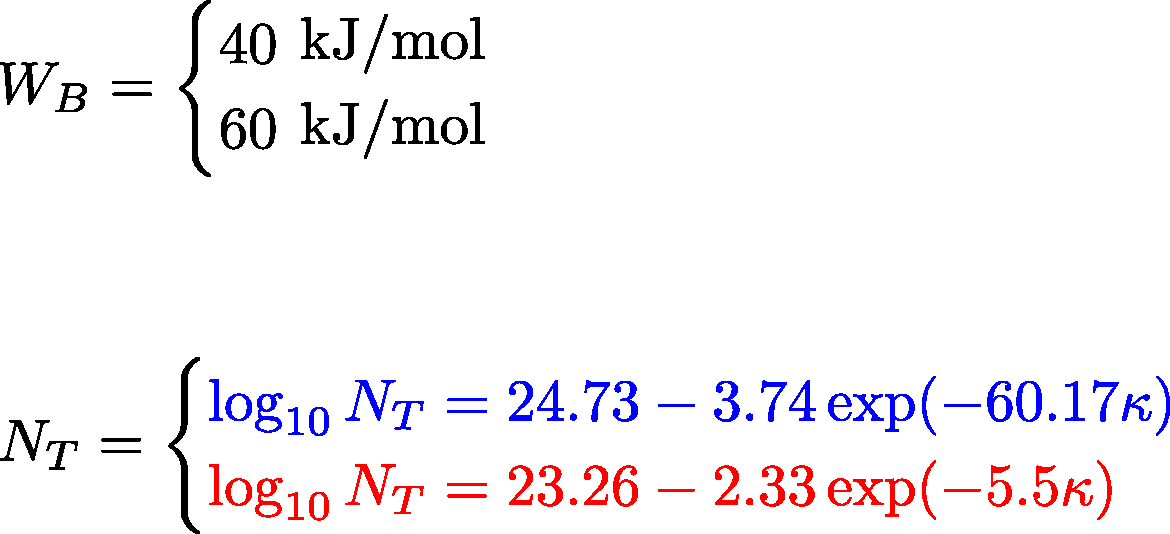
\includegraphics[width=0.95\textwidth]{Images/cases.pdf} \\
	\end{figure}
	\end{column}
	
	\begin{column}{0.45\textwidth}
	\begin{figure}
		\centering
		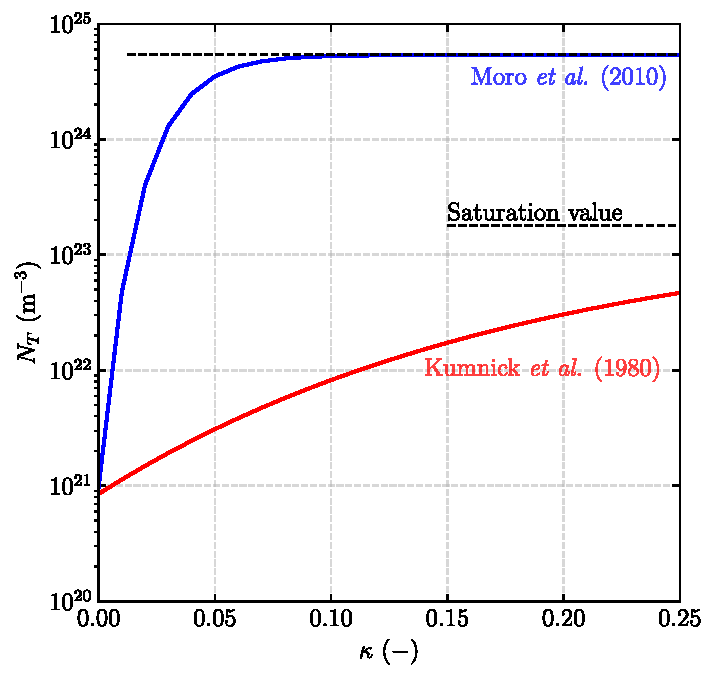
\includegraphics[width=1.0\textwidth]{Images/plot_NT_epcum.pdf} \\
	\end{figure}
	\end{column}
\end{columns}

\end{frame}

%%%%%%%%%%%%%%%%%%%%%%%%%%%%%%%%%%%%%%%%%%%%%%%%%%%%%%%%%%%

\begin{frame}{Hydrogen embrittled depth}

\begin{figure}
	\centering
	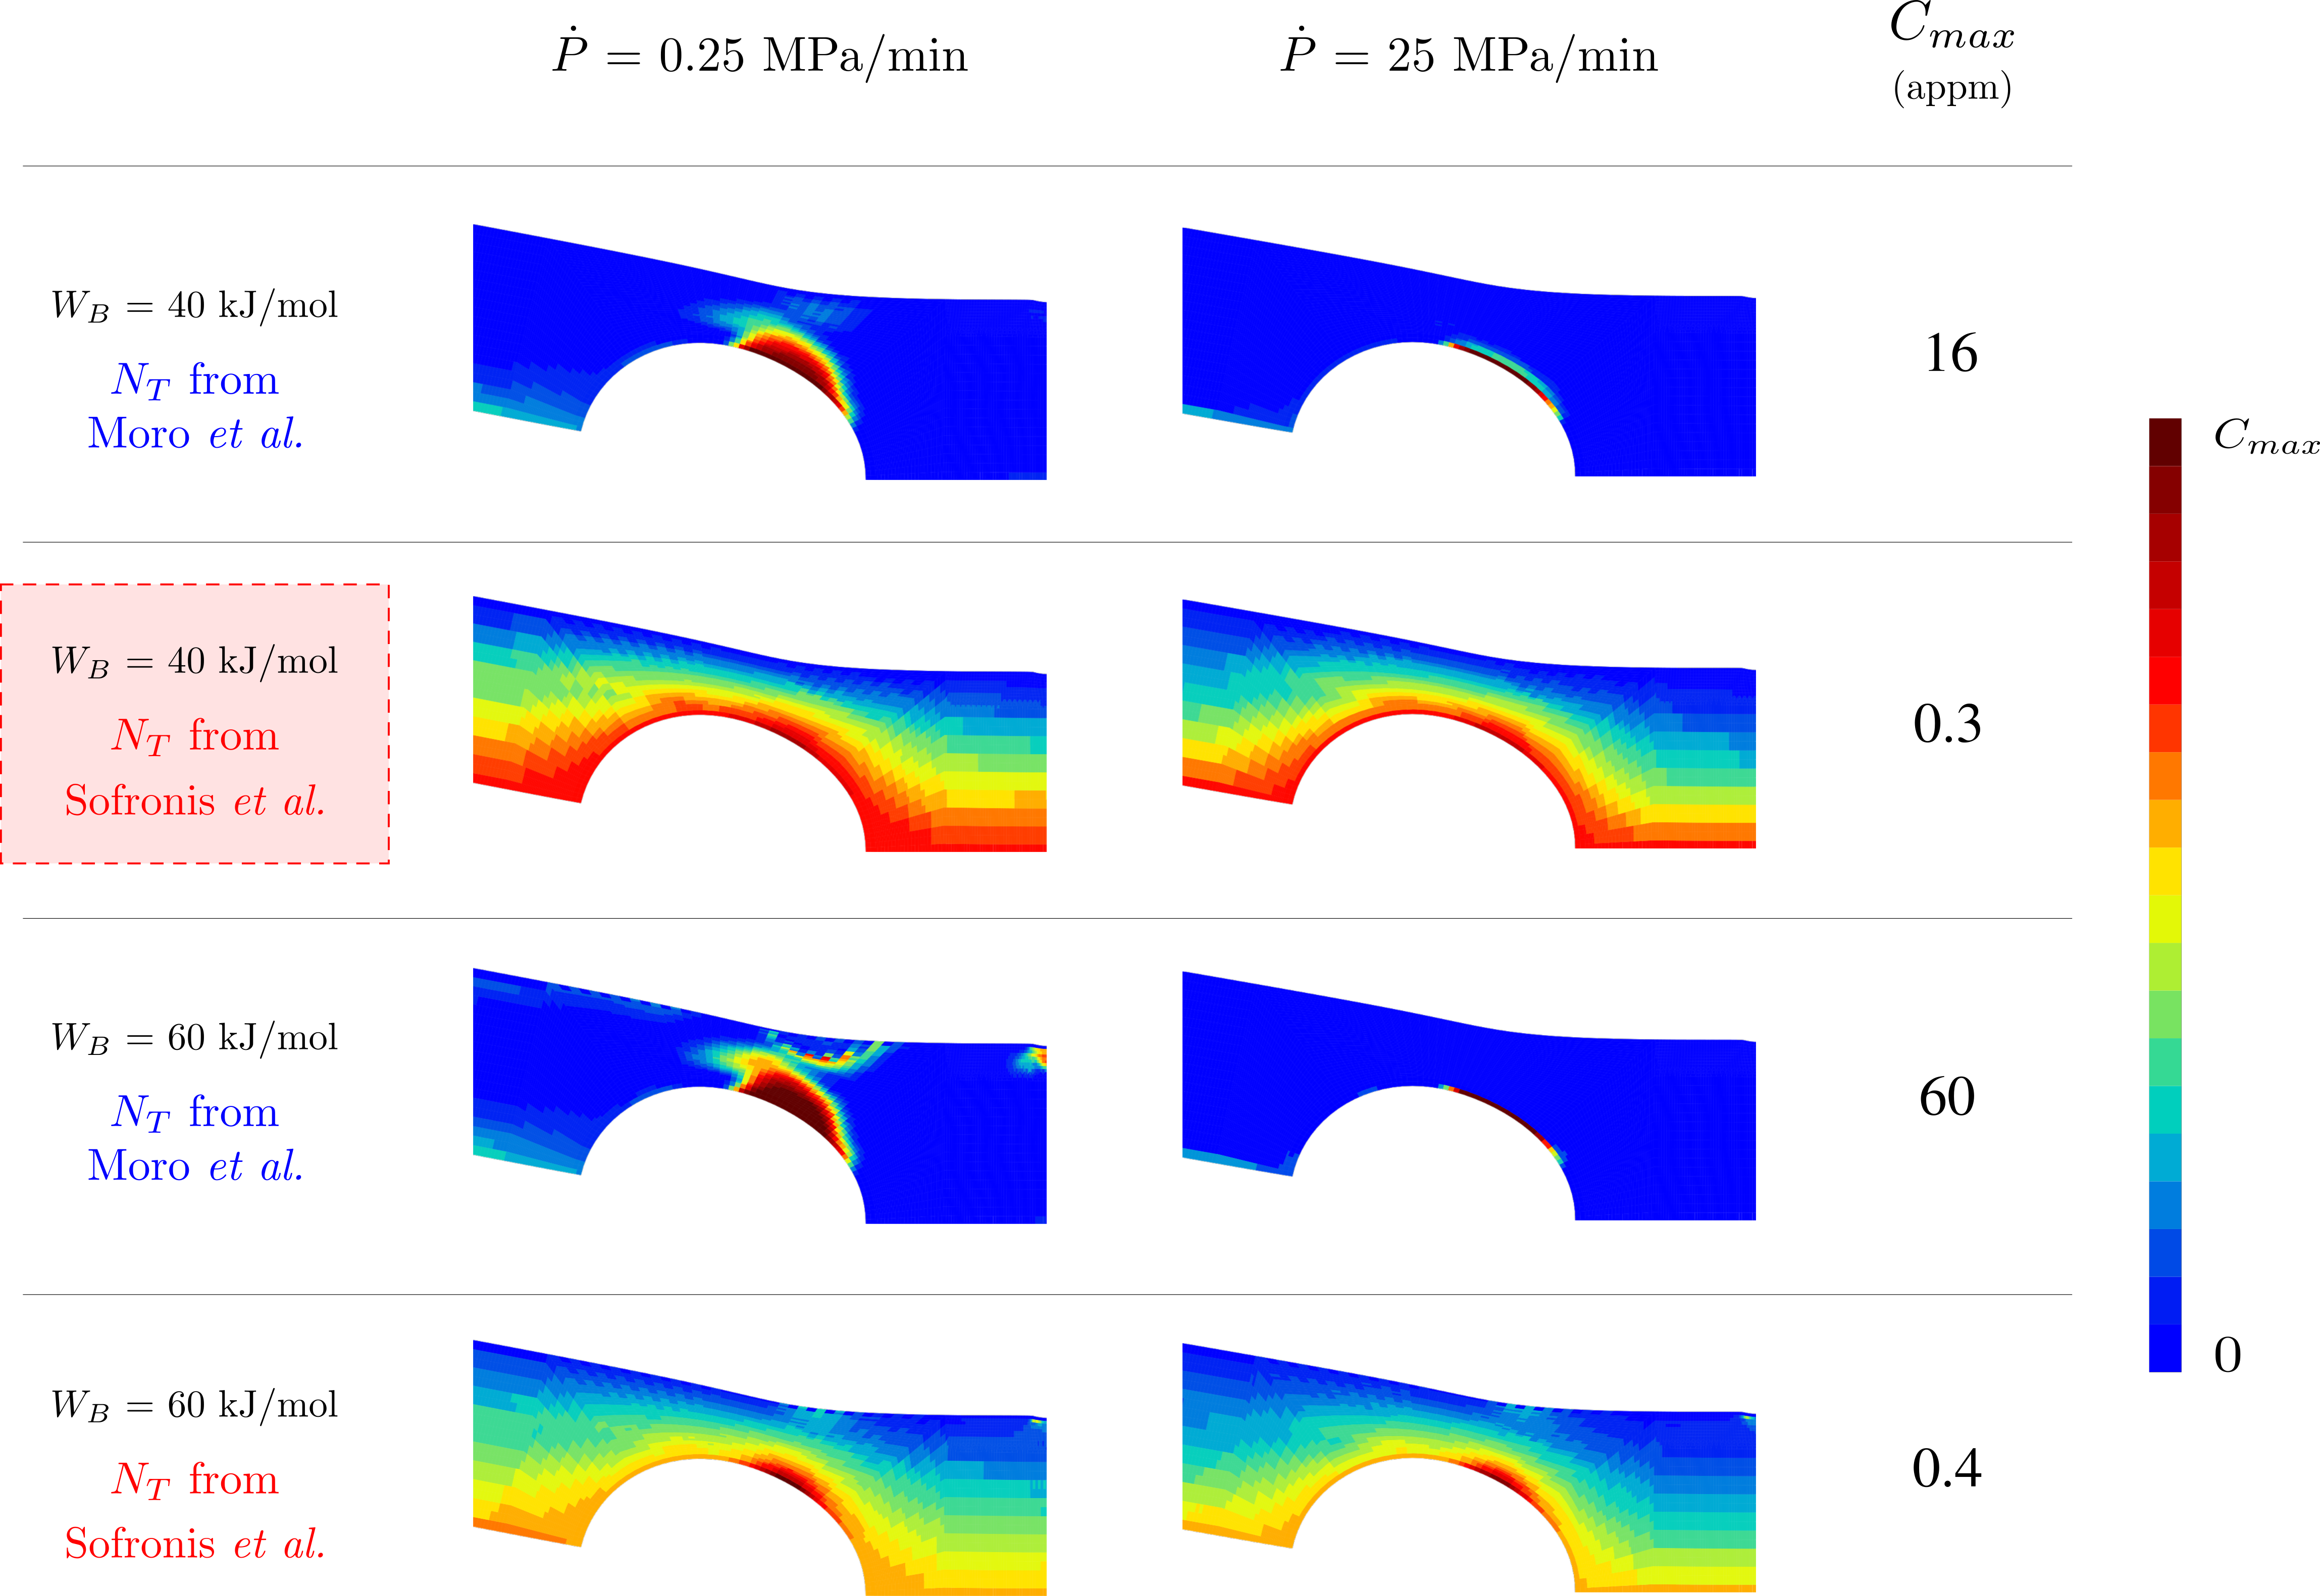
\includegraphics[width=0.9\textwidth]{Images/table_zoom.png} \\
\end{figure}

\end{frame}

%%%%%%%%%%%%%%%%%%%%%%%%%%%%%%%%%%%%%%%%%%%%%%%%%%%%%%%%%%%

\begin{frame}{Principal stress evolution}

\begin{itemize}
	\item Specimens that develop higher principal stress ($\sigma_I$) in the fracture zone fail at a lower hydrogen pressure ($P_a(H_2)$)
	\vspace{0.25cm}
	\item The total hydrogen concentration reduces the maximum principal stress that that triggers fracture
\end{itemize}

\begin{columns}

\begin{column}{0.49\textwidth}
	\begin{figure}
		\centering
		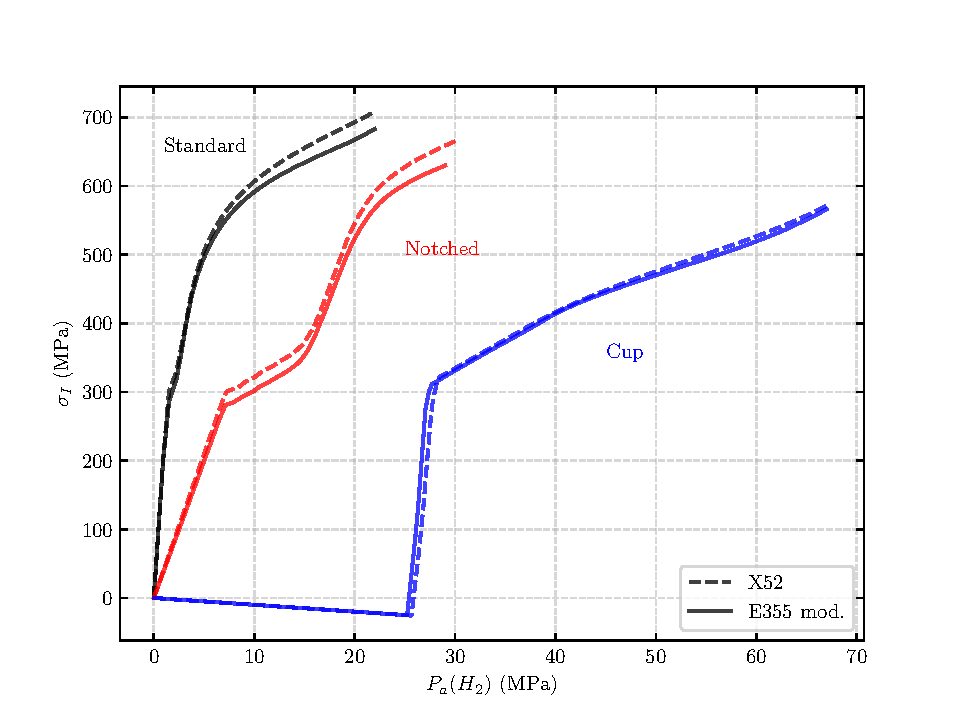
\includegraphics[width=\textwidth]{Images/sigp1_pressure.pdf} \\
	\end{figure}
\end{column}

\begin{column}{0.49\textwidth}
	\begin{figure}
		\centering
		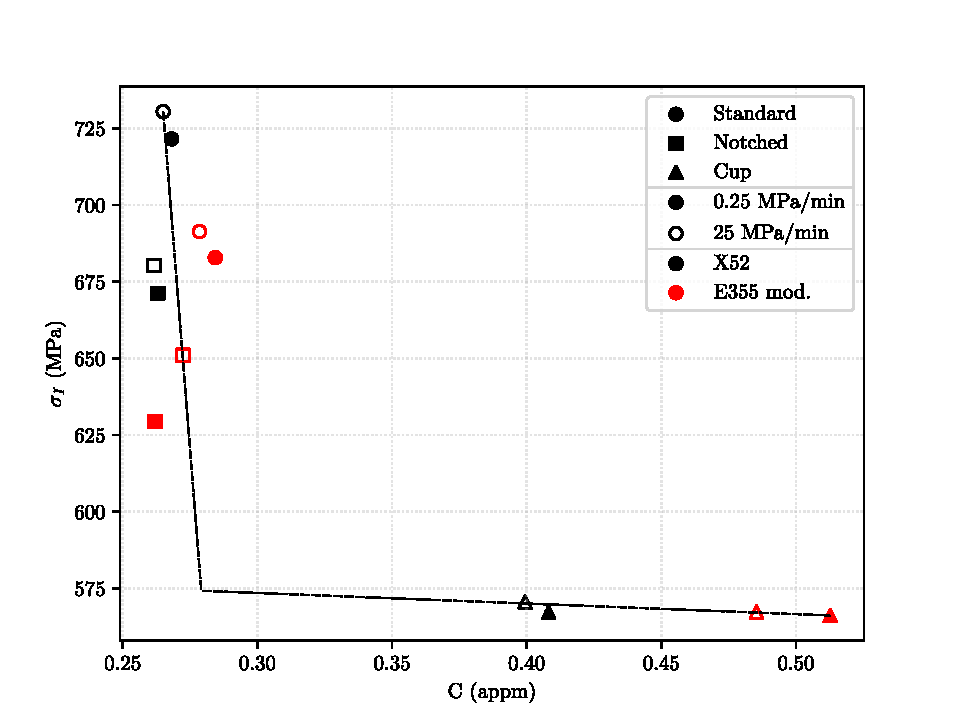
\includegraphics[width=\textwidth]{Images/plot_sigp1_C_edit.pdf} \\
	\end{figure}
\end{column}

\end{columns}

\end{frame}

%%%%%%%%%%%%%%%%%%%%%%%%%%%%%%%%%%%%%%%%%%%%%%%%%%%%%%%%%%%

%\subsection{Hydrogen uptake during a tensile test}
%
%\begin{frame}{Outline}
%	\tableofcontents[ 
%    currentsubsection, 
%    hideothersubsections, 
%    sectionstyle=show/shaded, 
%    subsectionstyle=show/shaded, 
%    ] 
%\end{frame}
%
%%%%%%%%%%%%%%%%%%%%%%%%%%%%%%%%%%%%%%%%%%%%%%%%%%%%%%%%%%%%
%
%\begin{frame}{Experimental procedure}
%
%\textbf{\textcolor{MINESBlue}{\large Tensile test:}}
%\vspace{0.1cm}
%\begin{itemize}
%	\item Material: X52 vintage steel
%	\vspace{0.1cm}
%	\item Gaseous atmosphere under different conditions:
%\vspace{0.1cm}
%\begin{table}[ht!]
%	\small
%    \centering
%    \renewcommand{\arraystretch}{1.5}
%    \begin{tabular}{ll}
%    \textbf{Environment}                 & Air, 85 bar H$_\text{2}$                               \\ \hline
%    \textbf{Strain}                 & 0\%, 30\%Rp02, 90\%Rp02, 3\%, 6\%, 12\%             \\ \hline
%    \textbf{Strain Rate (s$^{-1}$)} & $1\times10^{-5}$, $1\times10^{-4}$, $1\times10^{-3}$ \\ \hline
%    \textbf{Dwell}                       & No dwell, Dwell                                     
%    \end{tabular}
%\end{table}
%	
%\end{itemize}
%
%\begin{columns}
%
%\begin{column}{0.49\textwidth}
%	\begin{figure}
%		\centering
%		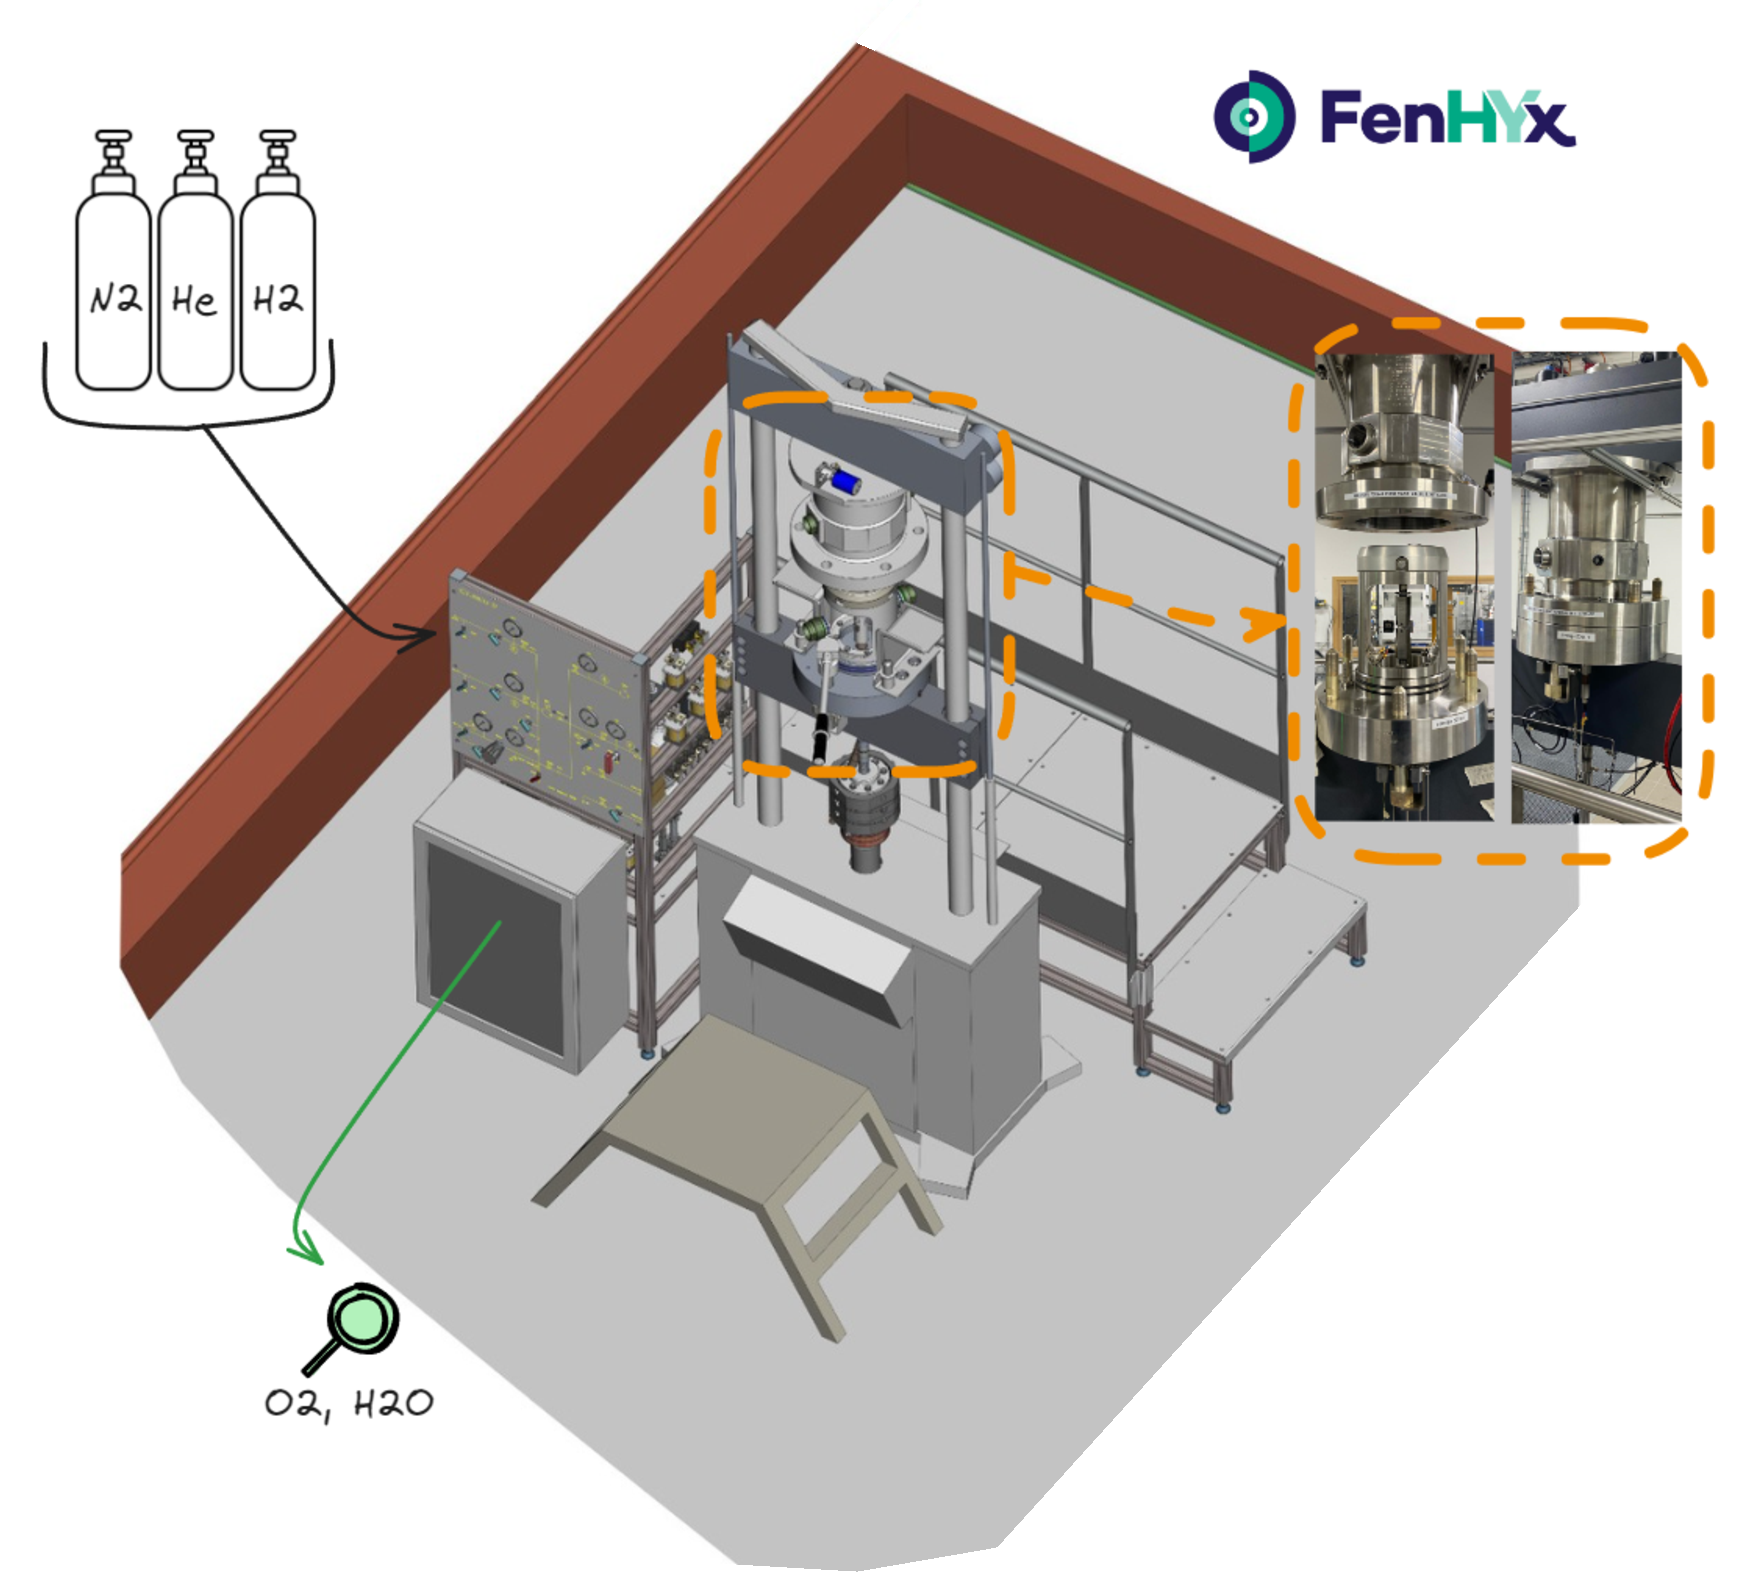
\includegraphics[width=0.8\textwidth]{Images/machine_fenhyx.pdf} \\
%	\end{figure}
%\end{column}
%
%\begin{column}{0.49\textwidth}
%	\begin{figure}
%		\centering
%		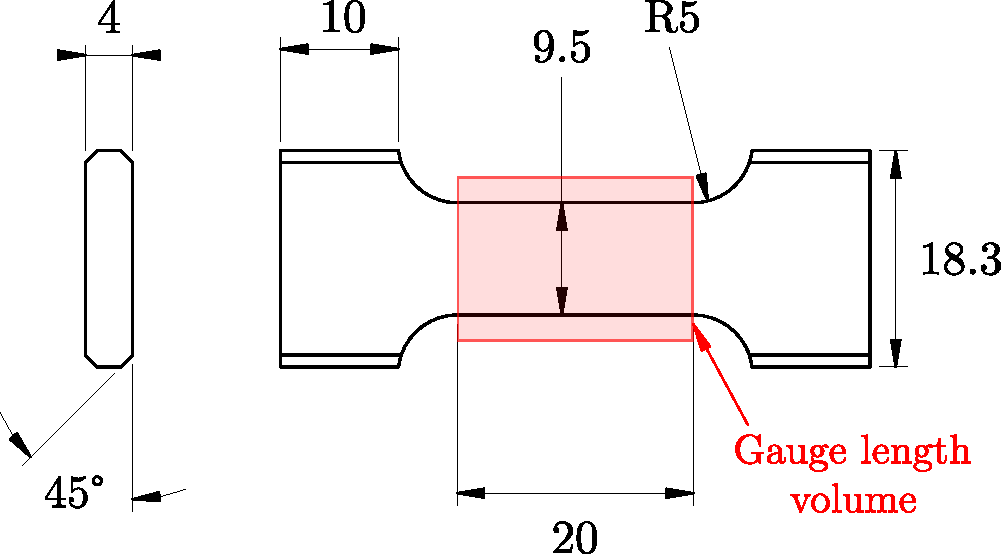
\includegraphics[width=0.9\textwidth]{Images/TDS_specimen.pdf} \\
%	\end{figure}
%\end{column}
%
%\end{columns}
%
%\end{frame}
%
%%%%%%%%%%%%%%%%%%%%%%%%%%%%%%%%%%%%%%%%%%%%%%%%%%%%%%%%%%%%
%
%\begin{frame}{Experimental procedure}
%
%\textbf{\textcolor{MINESBlue}{\large Thermal Desorption Spectroscopy (TDS) test:}}
%\vspace{0.15cm}
%\begin{itemize}
%	\item High precision (10$^{-3}$ wppm), calibration with a Certified Reference Material (CRM) with a known hydrogen mass
%	\vspace{0.15cm}
%	\item Temperature ramp of 10$^{\circ}$C/min up to 600$^{\circ}$C 
%	\vspace{0.15cm}
%	\item The hydrogen content is determined by integrating the first peak in the TDS spectra
%\end{itemize}
%
%\begin{figure}
%	\centering
%	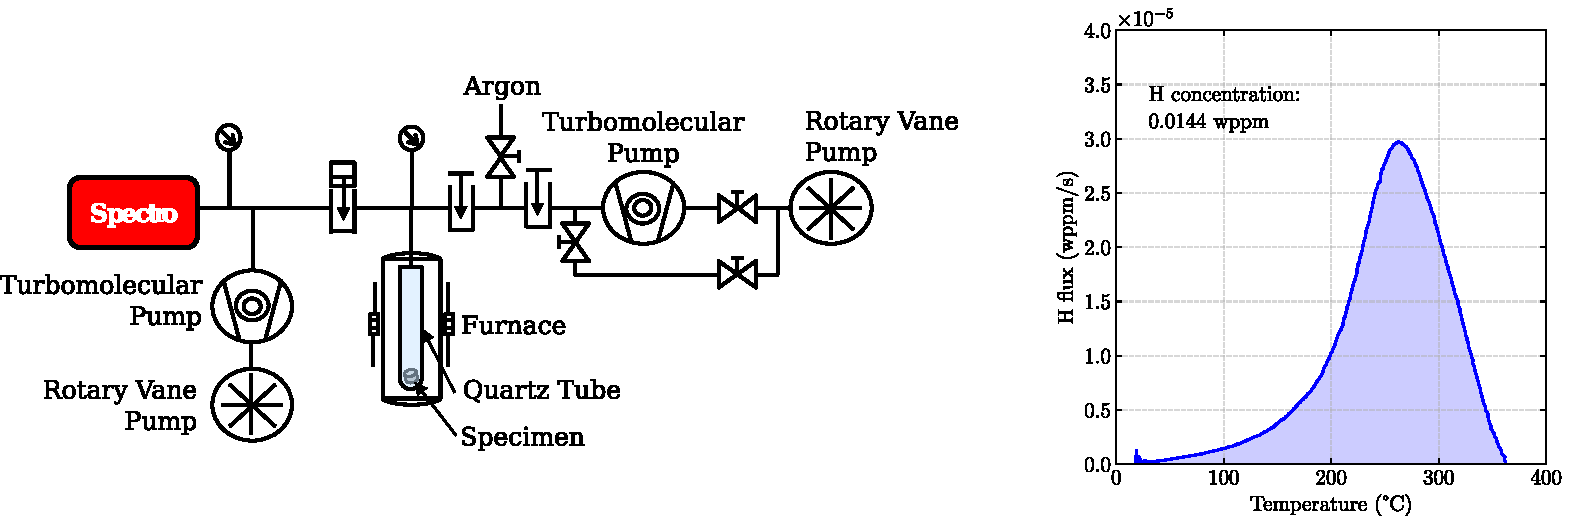
\includegraphics[width=0.95\textwidth]{Images/TDS_spectra.pdf} \\
%\end{figure}
%
%\end{frame}
%
%%%%%%%%%%%%%%%%%%%%%%%%%%%%%%%%%%%%%%%%%%%%%%%%%%%%%%%%%%%%
%
%\begin{frame}{Simulation model}
%
%\begin{columns}
%
%\begin{column}{0.65\textwidth}
%
%\begin{itemize}
%	\item 3D mesh of 1/8 of the specimen (plane strain)
%	\vspace{0.15cm}
%	\item Elasto(visco)-plastic behavior
%	\vspace{0.15cm}
%	\item Hydrogen applied to the exposed surfaces
%	\vspace{0.15cm}
%	\item $N_T(\kappa)$ adjusted based on experimental results at different strain levels
%\end{itemize}
%
%	\vspace{0.25cm}
%
%	\begin{figure}
%		\centering
%		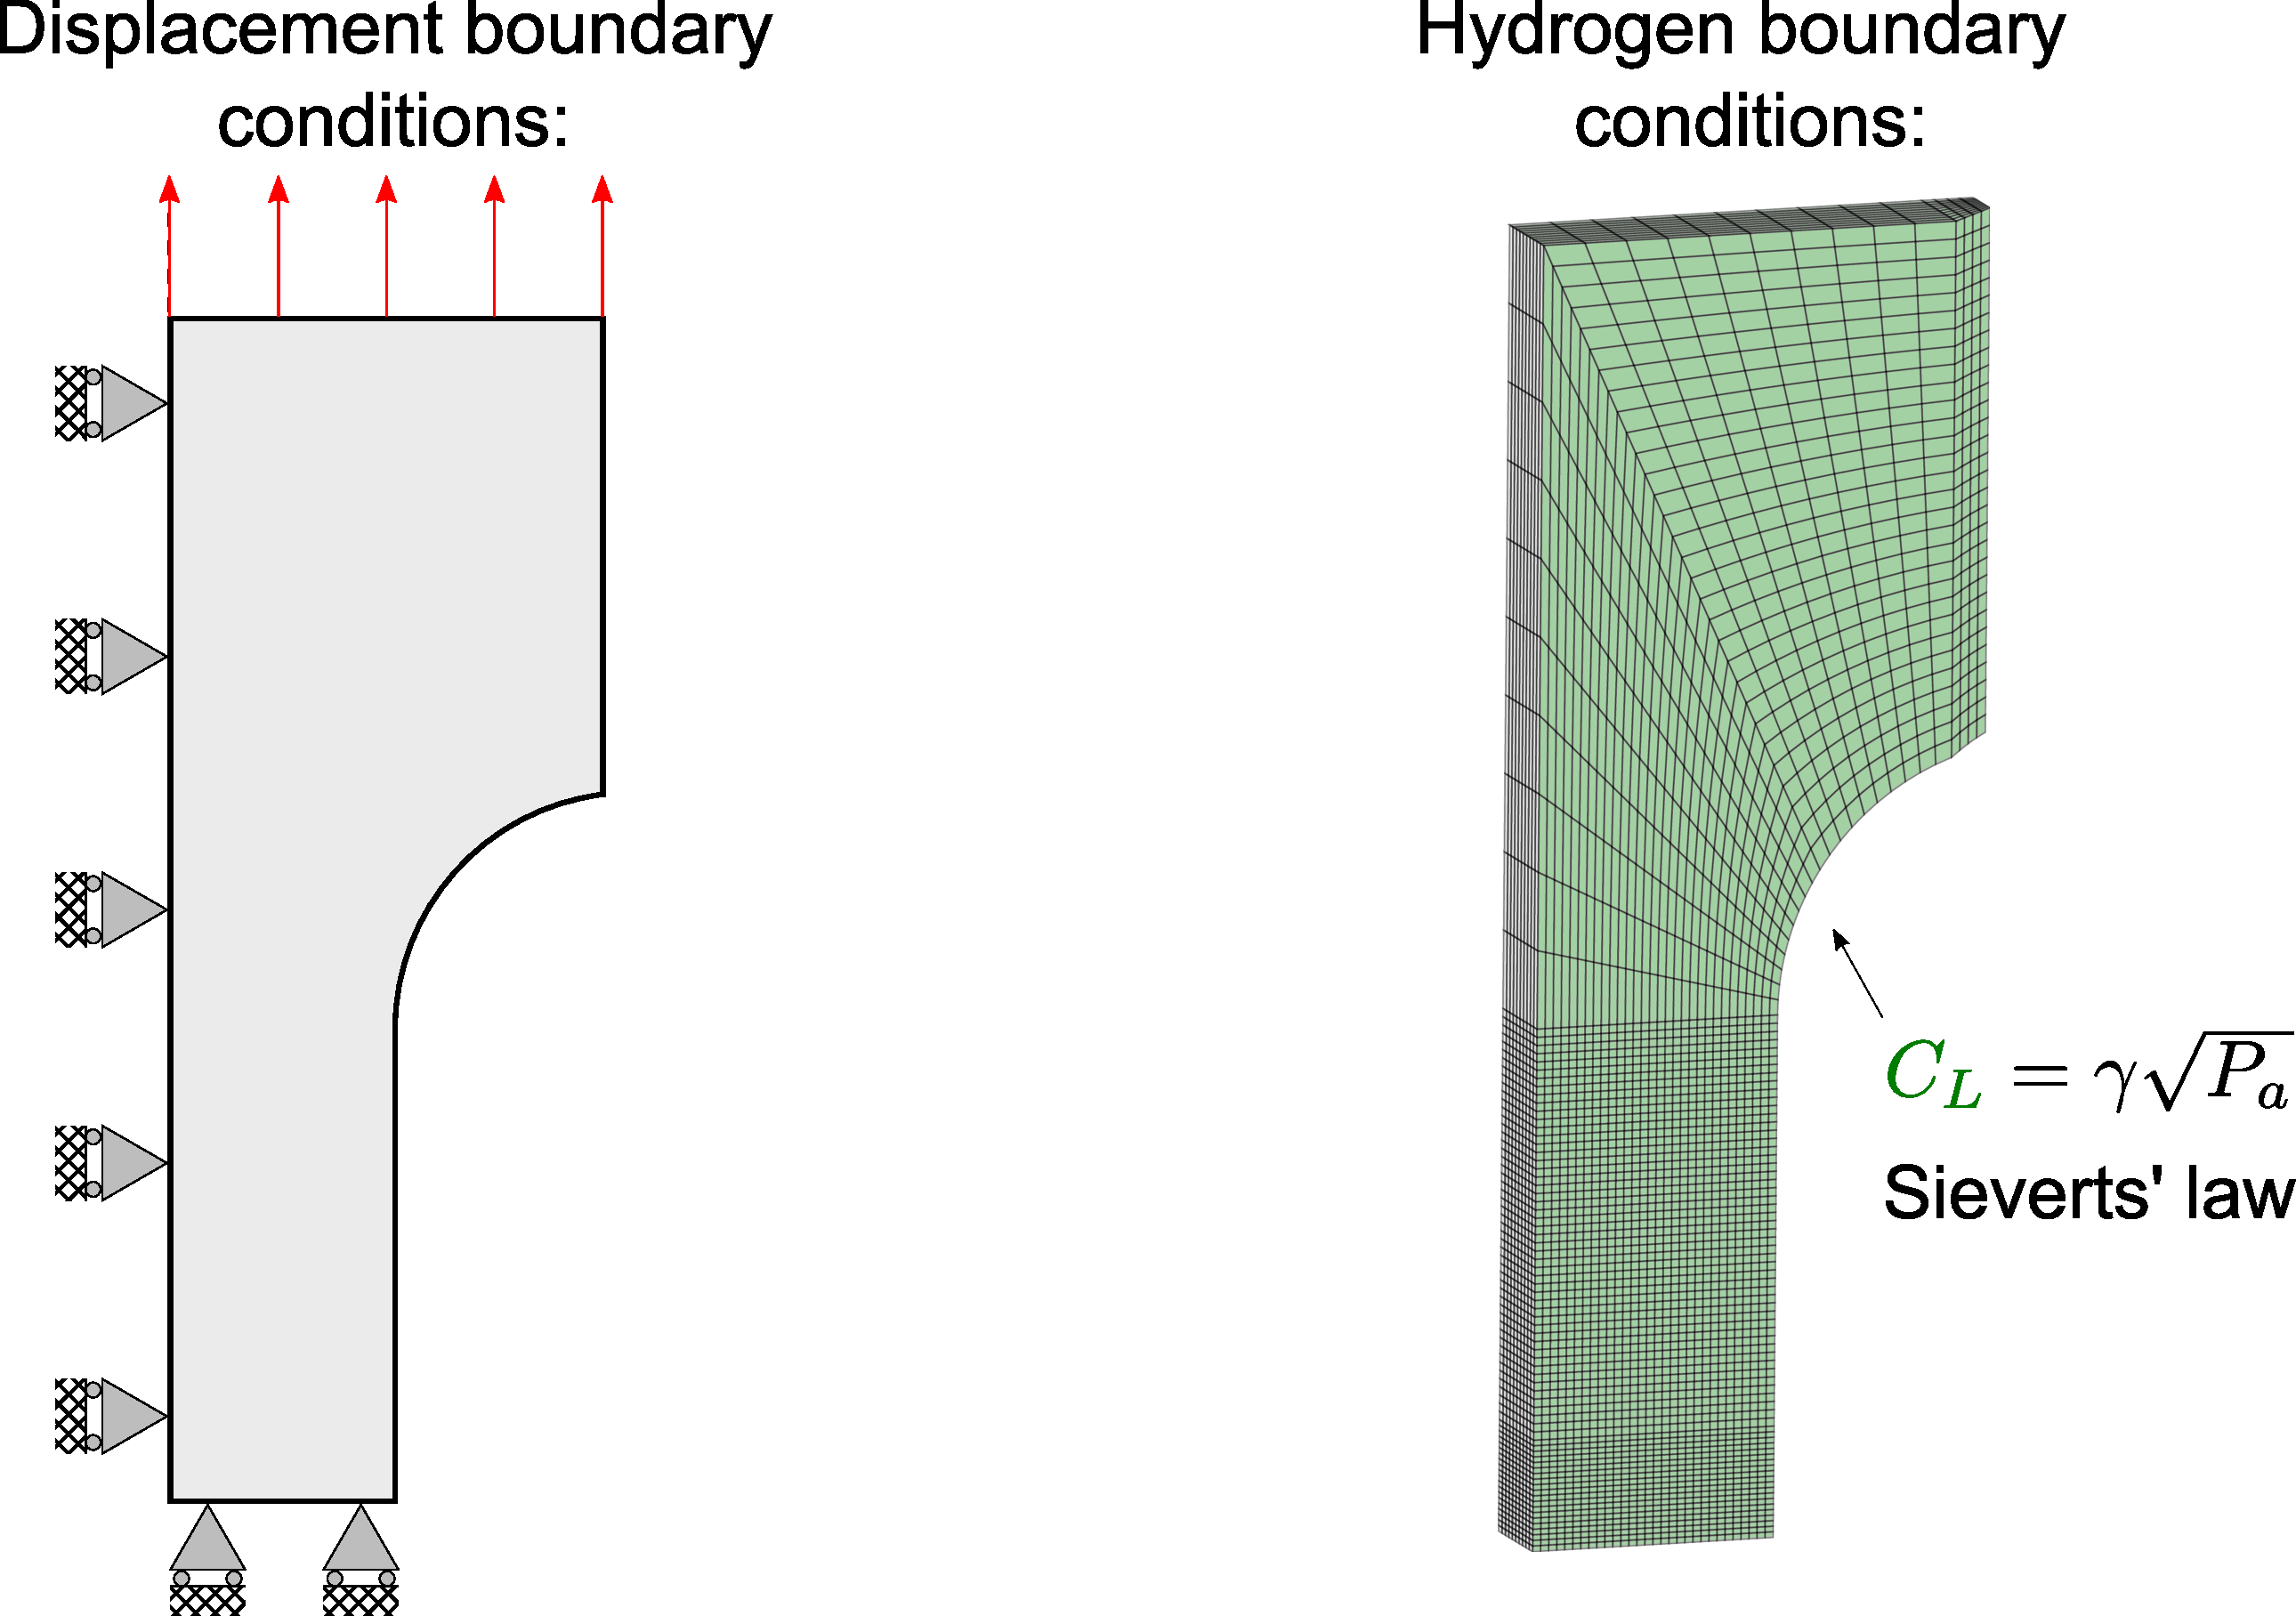
\includegraphics[width=0.8\textwidth]{Images/TDS_BC.pdf} \\
%	\end{figure}
%	
%	\vspace{0.15cm}
%
%\end{column}
%
%\begin{column}{0.35\textwidth}
%	\begin{figure}
%		\centering
%		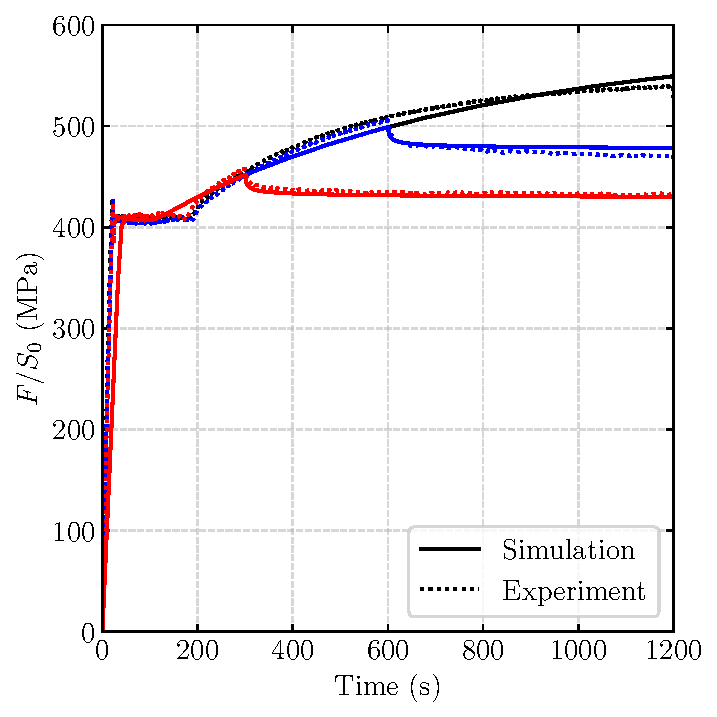
\includegraphics[width=0.99\textwidth]{Images/plot_time_stress.pdf} \\
%		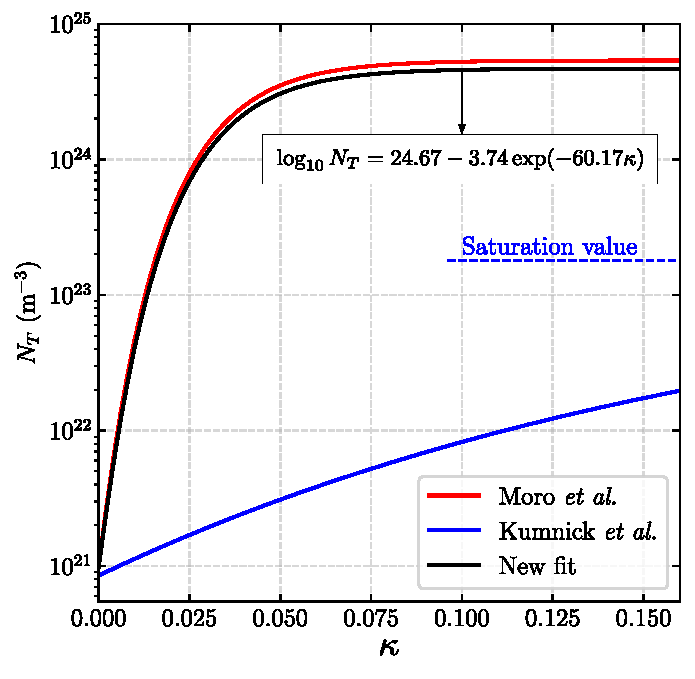
\includegraphics[width=0.95\textwidth]{Images/NT_TDS.pdf}
%	\end{figure}
%\end{column}
%
%\end{columns}
%
%\end{frame}
%
%%%%%%%%%%%%%%%%%%%%%%%%%%%%%%%%%%%%%%%%%%%%%%%%%%%%%%%%%%%%
%
%\begin{frame}{Strain effect}
%
%\begin{itemize}
%	\item Specimens deformed up to 90\%Rp02, 3\%, 6\% and 12\% at 
%	$\dot{\varepsilon} = 1\times10^{-4}$ s$^{-1}$
%	\vspace{0.15cm}
%	\item Higher strain levels lead to higher hydrogen concentrations
%	\vspace{0.15cm}
%	\item Most of hydrogen is located at the gauge length
%	\vspace{0.15cm}
%	\item For all cases, hydrogen is mostly located near the surface
%\end{itemize}
%
%\vspace{0.15cm}
%
%	\begin{figure}
%		\centering
%		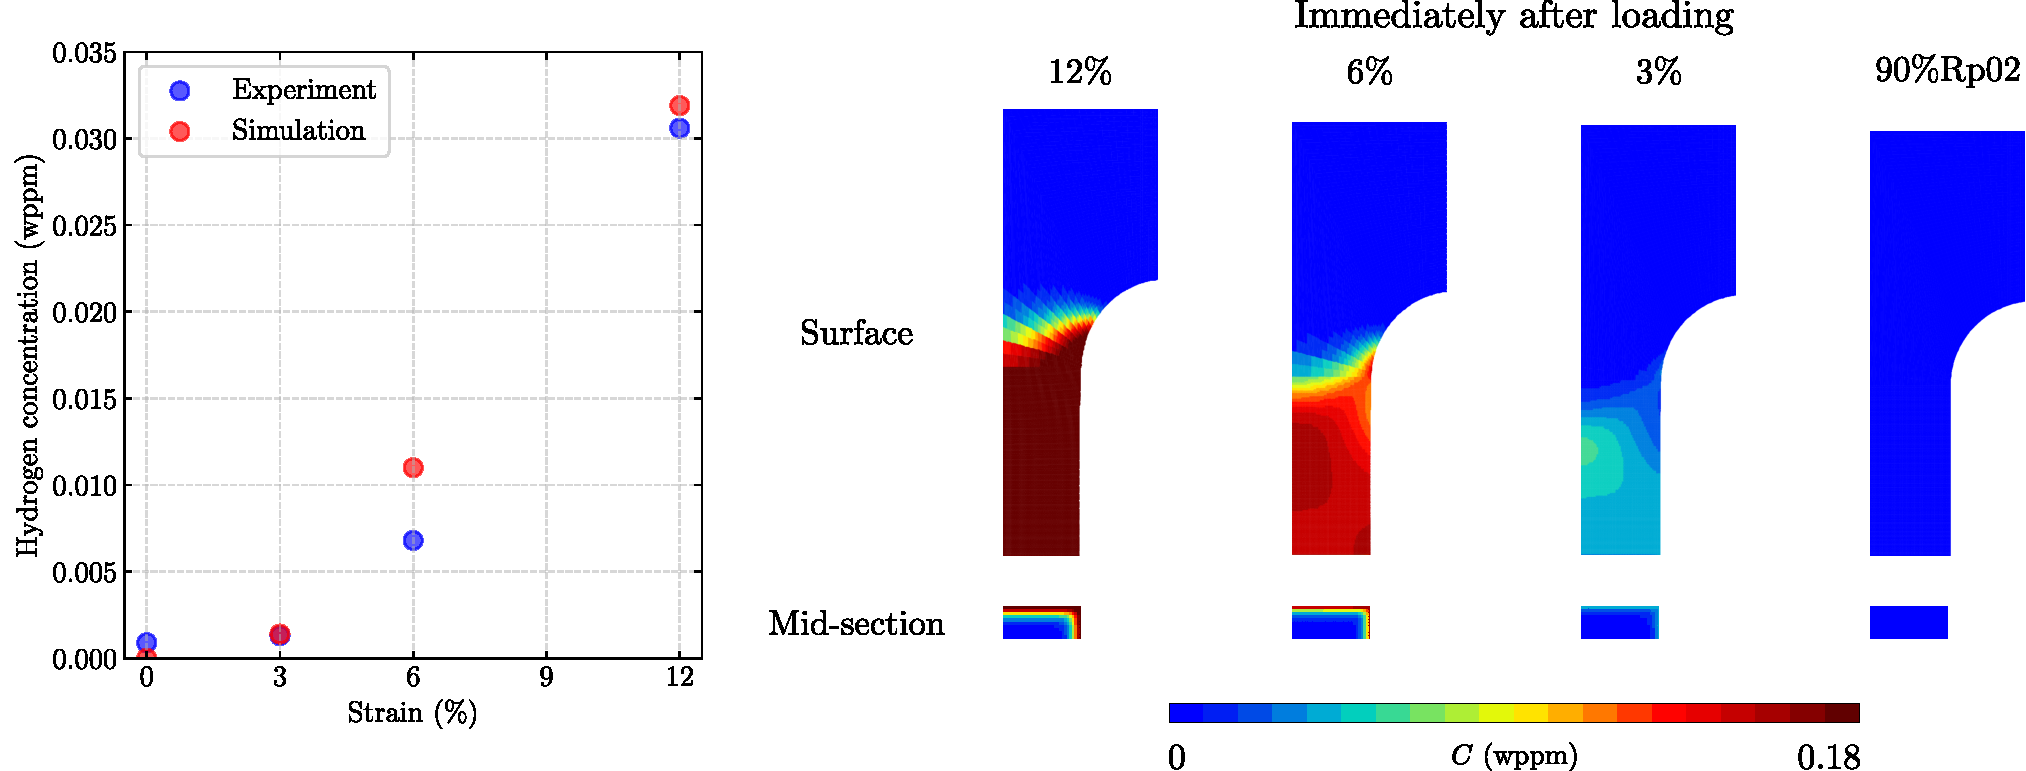
\includegraphics[width=\textwidth]{Images/strain_effect.pdf} \\
%	\end{figure}
%
%\end{frame}
%
%%%%%%%%%%%%%%%%%%%%%%%%%%%%%%%%%%%%%%%%%%%%%%%%%%%%%%%%%%%%
%
%\begin{frame}{Strain effect}
%
%	\begin{itemize}
%		\item The preparations required before the TDS test takes approximately \textbf{one hour}, at which hydrogen can freely desorb the specimen
%		\vspace{0.15cm}
%		\item The amount of hydrogen that leaves the specimen during resting is lower at higher strains
%		\vspace{0.15cm}
%		\item With the actual model, at least 80\% of the hydrogen content leaves the specimen during resting
%	\end{itemize}
%
%	\begin{figure}
%		\centering
%		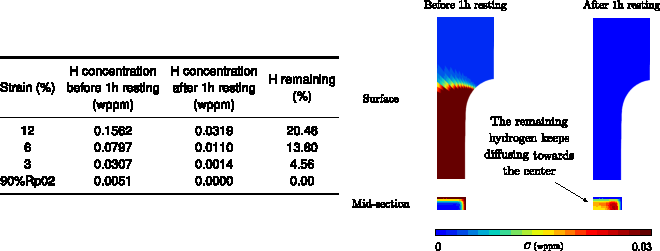
\includegraphics[width=\textwidth]{Images/resting_time.pdf} \\
%	\end{figure}
%
%\end{frame}
%
%
%%%%%%%%%%%%%%%%%%%%%%%%%%%%%%%%%%%%%%%%%%%%%%%%%%%%%%%%%%%%
%
%\begin{frame}{Strain rate effect}
%
%\begin{columns}
%
%\begin{column}{0.55\textwidth}
%\begin{itemize}
%	\item Tests conducted at three different strain rates: $1\times10^{-3}$, $1\times10^{-4}$ and $1\times10^{-5}$ s$^{-1}$
%	\vspace{0.25cm}
%	\item One-hour resting time allowing hydrogen desorption is considered
%	\vspace{0.25cm}
%	\item \textbf{Lower strain rates} lead to \textbf{higher hydrogen content}, as hydrogen has more time to diffuse throughout the material
%\end{itemize}
%\end{column}
%
%\begin{column}{0.45\textwidth}
%\begin{figure}
%	\centering
%	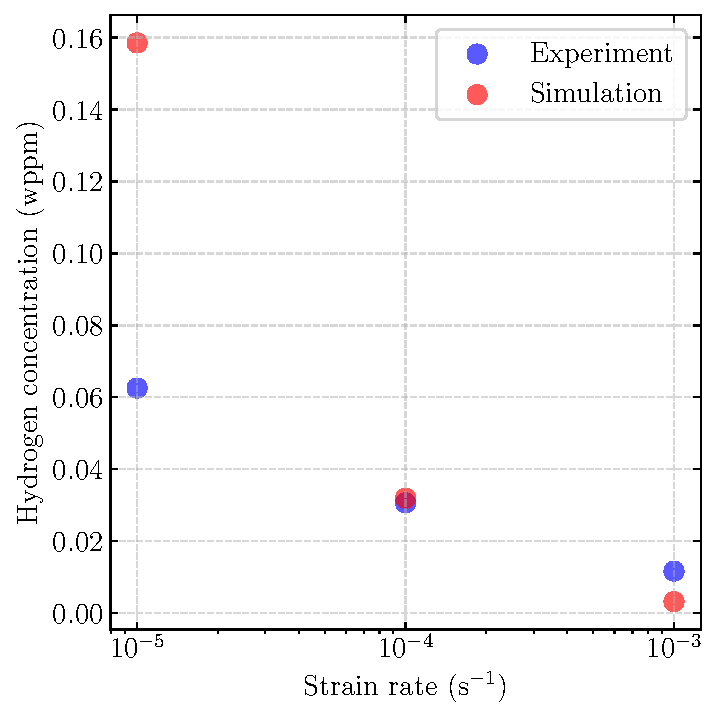
\includegraphics[width=0.9\textwidth]{Images/strain_rate_effect.pdf} \\
%	\vspace{0.25cm}
%%	\includegraphics[width=\textwidth]{Images/C_field_strain_rate_effect.pdf}
%\end{figure}
%
%\end{column}
%\end{columns}
%
%\begin{figure}
%		\centering
%		\includegraphics[width=0.65\textwidth]{Images/C_field_strain_rate_effect.pdf} \\
%	\end{figure}
%
%\end{frame}
%
%%%%%%%%%%%%%%%%%%%%%%%%%%%%%%%%%%%%%%%%%%%%%%%%%%%%%%%%%%%%
%
%\begin{frame}{Dwell effect}
%
%\begin{itemize}
%	\item \textbf{Dwell time:} the time a specimen is exposed to hydrogen without further deformation until it reaches the same exposure time as the most deformed specimen (12\%)
%	\vspace{0.25cm}
%	\item Specimens deformed up to 3\% strain at $1\times10^{-4}$ $1\times10^{-5}$ s$^{-1}$
%	\vspace{0.25cm}
%	\item Longer exposure $\rightarrow$ Higher hydrogen content
%\end{itemize}
%
%\begin{figure}
%	\centering
%	\includegraphics[width=\textwidth]{Images/Dwell_No_Dwell.pdf} 
%\end{figure}
%
%\end{frame}

%%%%%%%%%%%%%%%%%%%%%%%%%%%%%%%%%%%%%%%%%%%%%%%%%%%%%%%%%%%

\subsection{Hydrogen embrittlement modeling}

\begin{frame}{Outline}
	\tableofcontents[ 
    currentsubsection, 
    hideothersubsections, 
    sectionstyle=show/shaded, 
    subsectionstyle=show/shaded, 
    ] 
\end{frame}

%%%%%%%%%%%%%%%%%%%%%%%%%%%%%%%%%%%%%%%%%%%%%%%%%%%%%%%%%%%

\begin{frame}{Database and material coefficients}

    \begin{itemize}
        \item \textbf{Database}: Briottet \textit{et al.}, 2012 and Moro \textit{et al.}, 2010: \textit{Effect of gaseous hydrogen on the mechanical properties of steel}
        
        \vspace{0.15cm}

        \item \textbf{Material:} high-strength steel (API X80 grade) in an environment of hydrogen and neutral gas
        
        \vspace{0.15cm}   

    \end{itemize}
    
\begin{columns}

	\begin{column}{0.6\textwidth}

	\begin{itemize}

		\item As HE corresponds to \textbf{quasi-cleavage}, a \textbf{stress dependance} is introduced to the nucleation law
                
		\vspace{0.15cm}
                
        \item The function expressing the nucleation rate due to quasi-cleavage is:
                
		\begin{equation*}
                    \textcolor{NewRed}{B_n(C)} = \frac{\textcolor{DarkGreen}{B_0}}{\textcolor{DarkGreen}{\sigma_C^0}} (\sigma_I - (1-q_1 f_{*})\textcolor{blue}{\sigma_C})
		\end{equation*}

		\vspace{0.15cm}

		\item Hydrogen decreases the critical stress to trigger void nucleation
        
	\end{itemize}

	\end{column}
    
    \begin{column}{0.4\textwidth}

	\begin{figure}
		\begin{tabular}{c}
			\includegraphics[width=0.95\textwidth]{Images/plot_sig_c.pdf}
		\end{tabular}
	\end{figure}

	\begin{textblock}{5}(11.5,14.15)
		\textcolor{DarkGreen}{\footnotesize (Material parameters)}
	\end{textblock}

	\end{column}
    
\end{columns}

\end{frame}

%%%%%%%%%%%%%%%%%%%%%%%%%%%%%%%%%%%%%%%%%%%%%%%%%%%%%%%%%%%

\begin{frame}{Tensile tests}

    \begin{itemize}
        \item Tensile tests under different strain rates under hydrogen gas
        \vspace{0.15cm}
        \item Slower rates lead to important ductility losses
    \end{itemize}
    
    \begin{columns}
    
        \begin{column}{0.45\textwidth}
            \begin{figure}
                \begin{tabular}{c}
                    \includegraphics[width=0.9\textwidth]{Images/ST_specimen_Moro_BC.pdf}\\
                    \\
                    \includegraphics[width=0.8\textwidth]{Images/fracture_surface.png}\\
                \end{tabular}
            \end{figure}
            \centering \scriptsize \textcolor{gray}{(Experimental data: Briottet \textit{et al.}, 2012)}
        \end{column}
    
    
        \begin{column}{0.55\textwidth}
            \begin{figure}
                \begin{tabular}{c}
                    \includegraphics[width=0.6\textwidth]{Images/calcul_pl.pdf}\\
                    \\
                    \includegraphics[width=0.7\textwidth]{Images/fig_ST_sim_edt.pdf}\\
                \end{tabular}
            \end{figure} 
        \end{column}
    
    \end{columns}
    
\end{frame}

%%%%%%%%%%%%%%%%%%%%%%%%%%%%%%%%%%%%%%%%%%%%%%%%%%%%%%%%%%%

\begin{frame}{Tensile tests}

    \begin{itemize}
        \item Different damage evolution under hydrogen environment
        \vspace{0.15cm}
        \item Multicrack initiation on the surface
    \end{itemize}

    \vspace{4.5cm}

% ------------------------------------------------

\begin{tikzpicture}[remember picture, overlay]
    \node at (current page.south west) [xshift=4.5cm, yshift=4cm] {\includegraphics[width=0.7\textwidth]{Images/fig_ST_f_edt.pdf}}; 
\end{tikzpicture}

% ------------------------------------------------

    \begin{tikzpicture}[remember picture, overlay]
    
        \node at (current page.south west) [xshift=10.9cm, yshift=4.15cm]{
            \includemedia[
            % width=0.8\linewidth,height=0.6\linewidth, 
            width=0.3\textwidth,
            activate=onclick,
            passcontext, % Keep the \pause, etc. working in overlays
            addresource=Images/anim_surf_cracks/output.mp4, % chemin de votre fichier vidéo
            flashvars={
                source=Images/anim_surf_cracks/output.mp4   % chemin de votre fichier vidéo
                &autoPlay=true     % autoplay de la vidéo
                &loop=true         % lire en boucle
            }
        ]{\includegraphics[width=0.3\textwidth]{Images/anim_surf_cracks/anim0159.png}}{VPlayer.swf}};
    
    \end{tikzpicture}

\end{frame}

%%%%%%%%%%%%%%%%%%%%%%%%%%%%%%%%%%%%%%%%%%%%%%%%%%%%%%%%%%%

\begin{frame}{Pressurized disk tests}
    \textbf{Hydrogen effect:}

    \vspace{0.2cm}

    \begin{itemize}
        \item Lower pressure at rupture with decreased ductility
        \vspace{0.15cm}
        \item Higher hydrogen concentration in the rupture zone
    \end{itemize}

    \vspace{0.1cm}

    \begin{columns}

        \begin{column}{0.45\textwidth}

            \begin{figure}
                \begin{tabular}{c}
                    \includegraphics[width=0.95\textwidth]{Images/fig_disk_tP.pdf}\\
                \end{tabular}
            \end{figure}

        \end{column}
    
        \begin{column}{0.55\textwidth}
            \begin{figure}
                \begin{tabular}{c}
                    \includegraphics[width=0.95\textwidth]{Images/fig_iso_values_disk.pdf}\\
                \end{tabular}
            \end{figure}
        \end{column}
    
    \end{columns}
    
    \begin{tikzpicture}[remember picture, overlay]
    	\node at (current page.south west) [xshift=10.5cm, yshift=7cm] {\includegraphics[width=2.25cm]{Images/machine_DPT_2.jpg}}; 
    \end{tikzpicture}
    
\end{frame}

%%%%%%%%%%%%%%%%%%%%%%%%%%%%%%%%%%%%%%%%%%%%%%%%%%%%%%%%%%%

\begin{frame}{Pressurized disk tests}

    \textbf{Effect of the pressurization rate:}
    \vspace{0.15cm}

    \begin{itemize}
        \item Tests under different pressurization rates on H$_{\textrm{e}}$ and H$_2$ gases
        \vspace{0.15cm}
        \item \textbf{Lower pressurization rate} $\rightarrow$ \textbf{Higher embrittlement} since has a longer time to diffuse
    \end{itemize}

    \begin{columns}

        \begin{column}{0.5\textwidth}

            \begin{figure}
                \begin{tabular}{c}
                    \includegraphics[width=0.95\textwidth]{Images/fig_disk_Pr_edt.pdf}\\
                \end{tabular}
            \end{figure}

            \centering \hspace{0.9cm} \scriptsize \textcolor{gray}{(Experimental data: Briottet \textit{et al.}, 2012)}

        \end{column}
    
        \begin{column}{0.5\textwidth}
            \begin{figure}
                \begin{tabular}{c}
                    \includegraphics[width=0.95\textwidth]{Images/C_P_rate.pdf}\\
                \end{tabular}
            \end{figure}
        \end{column}
    
    \end{columns}   
    
\end{frame}

%%%%%%%%%%%%%%%%%%%%%%%%%%%%%%%%%%%%%%%%%%%%%%%%%%%%%%%%%%%

\begin{frame}{Fracture toughness tests}


    \begin{itemize}
        \item 2D Compact Tension (CT) specimen - \textit{plane strain}
        \vspace{0.1cm}
        \item Uniaxial imposed displacement
        \vspace{0.1cm}
        \item Environment: air and hydrogen (30 MPa)
        \vspace{0.1cm}
        \item Lattice concentration (\textcolor{DarkGreen}{$C_L$}) derived from Sieverts' law imposed on the newly formed crack
    \end{itemize}

    \vspace{0.25cm}

    \begin{columns}

        \begin{column}{0.4\textwidth}

            \begin{figure}
                \begin{tabular}{c}
                    \includegraphics[width=0.85\textwidth]{Images/CT_specimen.pdf}\\
                \end{tabular}
            \end{figure}

        \end{column}
    
        \begin{column}{0.6\textwidth}

        \begin{figure}
            \begin{tabular}{c}
                \includegraphics[width=0.9\textwidth]{Images/CT_BC.pdf}\\
            \end{tabular}
        \end{figure}

        \end{column}
    
    \end{columns}  

\end{frame}

%%%%%%%%%%%%%%%%%%%%%%%%%%%%%%%%%%%%%%%%%%%%%%%%%%%%%%%%%%%

\begin{frame}{Fracture toughness tests}

    \begin{itemize}
        \item Crack length: post-processing considering broken elements $f_* = 0.99 \times 1/q_1$
        \vspace{0.15cm}
        \item $J$-integral computation: ASTM E1820 standard considering the simulated Load-CMOD curve
    \end{itemize}

\vspace{5cm}

% --------------------------------------------------

\begin{tikzpicture}[remember picture, overlay]
    \node at (current page.south west) [xshift=3.cm, yshift=3.25cm] {\includegraphics[width=5.5cm]{Images/J_da.pdf}}; 
\end{tikzpicture}

% --------------------------------------------------

\begin{tikzpicture}[remember picture, overlay]
    
    \node at (current page.south west) [xshift=9.5cm, yshift=3.4cm]{
        \includemedia[
        width=0.5\textwidth,
        activate=onclick,
        passcontext, % Keep the \pause, etc. working in overlays
        addresource=Images/anim_CT/output.mp4, % chemin de votre fichier vidéo
        flashvars={
            source=Images/anim_CT/output.mp4   % chemin de votre fichier vidéo
            &autoPlay=true     % autoplay de la vidéo
            &loop=true         % lire en boucle
        }
    ]{\includegraphics[width=0.55\textwidth]{Images/CT_CL.pdf}}{VPlayer.swf}};

\end{tikzpicture}

\begin{textblock}{10}(8.5,6.6)
        \small Hydrogen diffusion through the crack lips:
    \end{textblock}
    
\end{frame}

%%%%%%%%%%%%%%%%%%%%%%%%%%%%%%%%%%%%%%%%%%%%%%%%%%%%%%%%%%%

\subsection{Simulation of fracture toughness tests}

\begin{frame}{Outline}
	\tableofcontents[ 
    currentsubsection, 
    hideothersubsections, 
    sectionstyle=show/shaded, 
    subsectionstyle=show/shaded, 
    ] 
\end{frame}

%%%%%%%%%%%%%%%%%%%%%%%%%%%%%%%%%%%%%%%%%%%%%%%%%%%%%%%%%%%

\begin{frame}{Materials and geometries}

    \begin{itemize}
        \item X52 vintage steel
        \vspace{0.15cm}
        \item Tube thickness: 7.92 mm
        \vspace{0.15cm}
        \item Tests using standard and sub-size specimens
        \vspace{0.15cm}
        \item Pre-cracking and side grooves with $B_n = 10\%B$ at each side
        \vspace{0.15cm}
        \item Experiments and simulations \textbf{without hydrogen}
    \end{itemize}
    
    \vspace{0.25cm}

    \begin{figure}
        \begin{tabular}{c}
            \includegraphics[width=0.9\textwidth]{Images/CT_mDCT_specimens_X52.pdf} \\
        \end{tabular}
    \end{figure}

\end{frame}

%%%%%%%%%%%%%%%%%%%%%%%%%%%%%%%%%%%%%%%%%%%%%%%%%%%%%%%%%%%

\begin{frame}{Internal length and mesh discretization}

    \begin{itemize}
        \item \textbf{Nonlocal GTN model with two internal lengths}: 
        \vspace{0.15cm}
        \begin{itemize}
        	\item $\ell_{\kappa}$: accumulated plastic strain (void nucleation)
        \vspace{0.15cm}
        \item $\ell_{\omega}$: plastic volume change (void growth)
        \end{itemize}
        \vspace{0.15cm}
        \item Typical element size used in nonlocal models for pipeline
steel simulations (\textcolor{gray}{Madi et al., 2020}): $\ell_{\omega} = 100$~$\mu$m
\vspace{0.15cm}
		\item The length scale associated with secondary nucleation is
likely smaller: $\ell_{\kappa} = 33$~$\mu$m
    \end{itemize}

    \vspace{0.7cm}

    \begin{columns}
        \column{0.48\textwidth}
        \centering
        \includegraphics[width=0.9\textwidth]{Images/nlgeom_si_ig.pdf}
        
        \column{0.48\textwidth}
        \centering
        \includegraphics[width=0.9\textwidth]{Images/internal_length.pdf}
    \end{columns}

\end{frame}

%%%%%%%%%%%%%%%%%%%%%%%%%%%%%%%%%%%%%%%%%%%%%%%%%%%%%%%%%%%

\begin{frame}{Crack propagation computation}

\begin{itemize}
	\item \textbf{Element removal technique}: an element of the mesh is removed when a predefined number of its integration points reach a critical porosity value:
	\vspace{0.15cm}
	$$ f_c = 1/q_1 - \epsilon$$	
	\vspace{0.05cm}
	\item \textbf{First method:} compliance technique $\rightarrow \Delta a$ is computed at the same way as in the experiments
	\vspace{0.15cm}
	\begin{itemize}
	\item \textbf{Drawback:} the load, hold, and unload steps into simulations significantly increases computation time
	\end{itemize}
\end{itemize}

\vspace{0.15cm}

\begin{figure}
        \begin{tabular}{c}
            \includegraphics[width=0.85\textwidth]{Images/plot_Load_CMOD_Tfake_edt.pdf} \\
        \end{tabular}
    \end{figure}

\end{frame}

%%%%%%%%%%%%%%%%%%%%%%%%%%%%%%%%%%%%%%%%%%%%%%%%%%%%%%%%%%%

\begin{frame}{Crack propagation computation}

\begin{itemize}
	\item \textbf{Second method:} Post-processing
	\vspace{0.15cm}
	\begin{itemize}
	\item The initial crack front is identified and the porosity values are analyzed on elements in the crack propagation zone
	\vspace{0.15cm}
	\item Elements with integration points reaching the critical porosity value ($f_c$) are considered broken. The crack front is updated after propagation.
	\end{itemize}
\end{itemize}

\begin{figure}
        \begin{tabular}{c}
            \includegraphics[width=0.99\textwidth]{Images/post_processing_technique.pdf} \\
        \end{tabular}
    \end{figure}

\end{frame}

%%%%%%%%%%%%%%%%%%%%%%%%%%%%%%%%%%%%%%%%%%%%%%%%%%%%%%%%%%%

\begin{frame}{Constituive law}

    \begin{itemize}
        \item The coefficients of the constitutive law were directly identified using the fracture toughness specimens
        \vspace{0.2cm}
        \item The hardening law is slightly different from the one previously presented $\rightarrow$ Dispersion observed for the X52 steel
        \vspace{0.2cm}
        \item Hardening law: 
        $$\sigma_F(\kappa) = \textrm{max}(340, 243 + 158 (1-\exp(-28.39 \kappa)) + 399 (1-\exp(-269 \kappa)))$$
        \item Damage coefficients:
        $$ q_1 = 1.25$$ 
        $$ q_2 =  1.40$$
        $$ \dot{f}_n = A_n (\bar{\kappa} > \kappa_c) \dot{\bar{\kappa}} \quad \textrm{with}$$ $$A_n = 1.0 \quad \textrm{and} \quad \kappa_c = 0.15 \rightarrow \textrm{\textbf{High and early void nucleation}}$$
    \end{itemize}

\end{frame}  

%%%%%%%%%%%%%%%%%%%%%%%%%%%%%%%%%%%%%%%%%%%%%%%%%%%%%%%%%%%

\begin{frame}{Results: simulations vs. experiments}

    \begin{itemize}
        \item Mesh dimensions precisely match the specimen dimensions for each test
        \vspace{0.15cm}
        \item An elasto-plastic model fails to accurately represent the fracture toughness test once crack propagation begins
        
    \end{itemize}

\begin{figure}
        \begin{tabular}{c}
            \includegraphics[width=0.95\textwidth]{Images/F_Load_X52.pdf} \\
        \end{tabular}
    \end{figure}
    
    \begin{textblock}{6}(6.5,13.25)
        \textcolor{gray}{\scriptsize (Experimental data: L. Santana)}
    \end{textblock}

\end{frame}  

%%%%%%%%%%%%%%%%%%%%%%%%%%%%%%%%%%%%%%%%%%%%%%%%%%%%%%%%%%%

\begin{frame}{Results: simulations vs. experiments}

\begin{itemize}
	\item Relatively low toughness values
	\vspace{0.1cm}
    \item Crack propagation initiates later for the simulations $\rightarrow$ This delay was partially addressed by reducing the void nucleation threshold
    \vspace{0.1cm}
    \item $J$ and $\delta$ (CTOD) values increase as specimen size decreases
\end{itemize}

\begin{columns}
    \column{0.48\textwidth}
    \centering
    \includegraphics[width=0.9\textwidth]{Images/plot_J-da_ALL_X52.pdf}
    
    \column{0.48\textwidth}
    \centering
    \includegraphics[width=0.9\textwidth]{Images/plot_CTOD-da_ALL_X52.pdf}
\end{columns}

	\begin{textblock}{6}(6.35,14.75)
        \textcolor{gray}{\scriptsize (Experimental data: L. Santana)}
    \end{textblock}

\end{frame}

%%%%%%%%%%%%%%%%%%%%%%%%%%%%%%%%%%%%%%%%%%%%%%%%%%%%%%%%%%%

\begin{frame}{Results: simulations vs. experiments}

    \begin{columns}
        \column{0.33\textwidth}
        \centering
        \includegraphics[width=1.0\textwidth]{Images/plot_J-da_mDCT2_X52.pdf}
        
        \column{0.33\textwidth}
        \centering
        \includegraphics[width=1.0\textwidth]{Images/plot_J-da_mDCT5_X52.pdf}

        \column{0.33\textwidth}
        \centering
        \includegraphics[width=1.0\textwidth]{Images/plot_J-da_CT_X52.pdf}
    \end{columns}

    \begin{figure}
        \begin{tabular}{c}
            \includegraphics[width=0.8\textwidth]{Images/tab_J-da.pdf} \\
        \end{tabular}
    \end{figure}

    \begin{textblock*}{7cm}(3.25cm,8.7cm)
        \small Construction line: $J = 2 \sigma_Y \Delta a$ (ASTM E1820)
    \end{textblock*}

\end{frame}

%%%%%%%%%%%%%%%%%%%%%%%%%%%%%%%%%%%%%%%%%%%%%%%%%%%%%%%%%%%

\begin{frame}{Results: simulations vs. experiments}

    \begin{columns}
        \column{0.33\textwidth}
        \centering
        \includegraphics[width=1.0\textwidth]{Images/plot_CTOD-da_mDCT2_X52.pdf}
        
        \column{0.33\textwidth}
        \centering
        \includegraphics[width=1.0\textwidth]{Images/plot_CTOD-da_mDCT5_X52.pdf}

        \column{0.33\textwidth}
        \centering
        \includegraphics[width=1.0\textwidth]{Images/plot_CTOD-da_CT_X52.pdf}
    \end{columns}

    \begin{figure}
        \begin{tabular}{c}
            \includegraphics[width=0.8\textwidth]{Images/tab_CTOD-da.pdf} \\
        \end{tabular}
    \end{figure}

    \begin{textblock*}{7cm}(3.25cm,8.7cm)
        \small Construction line: $\delta = 1.4 \Delta a$ (ASTM E1820)
    \end{textblock*}

\end{frame}

%%%%%%%%%%%%%%%%%%%%%%%%%%%%%%%%%%%%%%%%%%%%%%%%%%%%%%%%%%%

\begin{frame}{Parametrical study}

\textcolor{MINESBlue}{\textbf{Homothetic specimens:}}
\vspace{0.15cm}
    \begin{itemize}
        \item \textbf{Homothetic CT specimens} $\rightarrow$ Dimensions scaled systematically from the smallest to the largest
        \vspace{0.15cm}
        \item $B/W = 0.5$ and $a_0/W = 0.55$ for all cases
        \vspace{0.15cm}
        \item Each mesh was generated individually, ensuring correct element size with respect to the internal length
    \end{itemize}

    \vspace{4cm}
    
    \begin{textblock*}{11cm}(2cm,5cm)
        \only<1>{\includegraphics[width=0.9\textwidth]{Images/tab_homo.pdf}}
        \only<2>{\includegraphics[width=0.9\textwidth]{Images/tab_homo_2.pdf}}
    \end{textblock*}


\end{frame}

%%%%%%%%%%%%%%%%%%%%%%%%%%%%%%%%%%%%%%%%%%%%%%%%%%%%%%%%%%%

\begin{frame}{Parametrical study}

\textcolor{MINESBlue}{\textbf{Varying thickness:}}
\vspace{0.3cm}
\begin{itemize}
        \item \textbf{Varying thickness} $\rightarrow$ Specimen with the dimensions corresponding to a CT-12.5 with different thickness values
    \end{itemize}

    \vspace{0.5cm}

    \begin{columns}
        \column{0.48\textwidth}
        \centering
        \includegraphics[width=0.87\textwidth]{Images/geo_size_effect.pdf}
        
        \column{0.48\textwidth}
        \centering
        \includegraphics[width=0.9\textwidth]{Images/tab_size_effect.pdf}
    \end{columns}

\end{frame}

%%%%%%%%%%%%%%%%%%%%%%%%%%%%%%%%%%%%%%%%%%%%%%%%%%%%%%%%%%%

\begin{frame}{Parametrical study}

    \begin{itemize}
    	\item Coefficients identified for the X52 steel
    	\vspace{0.2cm}
        \item \textbf{Homothetic specimens:} Minor effect on toughness
        \vspace{0.2cm}
        \item \textbf{Varying thickness:} Toughness decreased with thickness
    \end{itemize}

    \vspace{0.15cm}

    \begin{columns}
        \column{0.48\textwidth}
        \centering
        \includegraphics[width=0.9\textwidth]{Images/plot_homo_Jda_1_2__1_4.pdf}
        
        \column{0.48\textwidth}
        \centering
        \includegraphics[width=0.9\textwidth]{Images/plot_12_5_Jda_1_2__1_4.pdf}
    \end{columns}

    \begin{textblock*}{5cm}(2.2cm,8.75cm)
        \small Homothetic specimens
    \end{textblock*}

    \begin{textblock*}{5cm}(8.5cm,8.75cm)
        \small Varying thickness
    \end{textblock*}

\end{frame}

%%%%%%%%%%%%%%%%%%%%%%%%%%%%%%%%%%%%%%%%%%%%%%%%%%%%%%%%%%%

\begin{frame}{Parametrical study}

	\vspace{0.25cm}

    \begin{itemize}
        \item Size and thickness effect on $J_{0.2}$ and $J_{0.5}$
        \vspace{0.15cm}
        \item Fracture toughness and thickness\\ do not have a bijective relationship
    \end{itemize}

    \vspace{0.15cm}

    \begin{columns}
        \column{0.48\textwidth}
        \centering
        \includegraphics[width=0.9\textwidth]{Images/plot_geoJ_homo_1_2__1_4.pdf}
        
        \column{0.48\textwidth}
        \centering
        \includegraphics[width=0.9\textwidth]{Images/plot_geoJ_12_5_1_2__1_4.pdf}
    \end{columns}

    \begin{textblock*}{3cm}(7.85cm,1.25cm) % Taille et position de l'image
        \includegraphics[width=3.5cm]{Images/bump.pdf}
    \end{textblock*}

    \begin{textblock*}{5cm}(2.2cm,8.75cm)
        \small Homothetic specimens
    \end{textblock*}

    \begin{textblock*}{5cm}(8.5cm,8.75cm)
        \small Varying thickness
    \end{textblock*}
    
\end{frame}

%%%%%%%%%%%%%%%%%%%%%%%%%%%%%%%%%%%%%%%%%%%%%%%%%%%%%%%%%%%

\begin{frame}{Parametrical study}

	\textcolor{MINESBlue}{\textbf{Varying damage coefficients:}}
	\vspace{0.3cm}
    \begin{itemize}
        \item \textbf{Hardening law:} same as the X52
        \vspace{0.5cm}
        \item \textbf{GTN's coefficients:}
        \vspace{0.2cm}
        \begin{itemize}
            \item $q_1 = 1.5$, $q_2 = 1.0$ $\rightarrow$ \textbf{Most ductile case}
            \vspace{0.2cm}
            \item $q_1 = 1.9$, $q_2 = 1.0$
            \vspace{0.2cm}
            \item $q_1 = 2.0$, $q_2 = 1.5$ $\rightarrow$ \textbf{Less ductile case}
        \end{itemize}
        \vspace{0.4cm}
        \item $\uparrow q_1$: increases void growth sensitivity, causing earlier growth and \textbf{reduced ductility}
        \vspace{0.2cm}
        \item $\uparrow q_2$: Leads to early crack initiation, \textbf{reduced ductility}, and abrupt fracture
        \vspace{0.2cm}
        \item \textbf{Low void nucleation:} $A_n$ = 0.2 and $\kappa_c$ = 0.8
    \end{itemize}

\end{frame}

%%%%%%%%%%%%%%%%%%%%%%%%%%%%%%%%%%%%%%%%%%%%%%%%%%%%%%%%%%%

\begin{frame}{Parametrical study}

	\textcolor{MINESBlue}{\textbf{Varying damage coefficients:}}
	\vspace{0.1cm}
	\normalsize
	\begin{itemize}
		\item Homothetic specimens exhibit more stable toughness values
		\vspace{0.1cm}
		\item More ductile material present more size effects
		\vspace{0.1cm}
		\item Even tests considered valid according to the standard can still display size effects
		\vspace{0.1cm}
		\item No bijective relationship between toughness and thickness
	\end{itemize}
	
    \begin{columns}
        \column{0.48\textwidth}
        \centering
        \includegraphics[width=0.75\textwidth]{Images/plot_comp_homo_q1_q2.pdf}
        
        \column{0.48\textwidth}
        \centering
        \includegraphics[width=0.75\textwidth]{Images/plot_comp_12_5_q1_q2.pdf}
    \end{columns}
    
    \begin{textblock*}{5cm}(2.2cm,8.95cm)
        \small Homothetic specimens
    \end{textblock*}

    \begin{textblock*}{5cm}(8.65cm,8.95cm)
        \small Varying thickness
    \end{textblock*}
    
\end{frame}

%%%%%%%%%%%%%%%%%%%%%%%%%%%%%%%%%%%%%%%%%%%%%%%%%%%%%%%%%%%

\section{Conclusions and perspectives}

\begin{frame}{Outline}
	\tableofcontents[ 
    currentsubsection, 
    hideothersubsections, 
    sectionstyle=show/shaded, 
    subsectionstyle=show/shaded, 
    ] 
\end{frame}

%%%%%%%%%%%%%%%%%%%%%%%%%%%%%%%%%%%%%%%%%%%%%%%%%%%%%%%%%%%

\begin{frame}{Conclusions}

\begin{itemize}

	\item \textbf{Comprehensive HE modeling:} Developed a numerical framework integrating hydrogen diffusion, plasticity, and damage mechanisms.
	\vspace{0.15cm}
	\item \textbf{Modified nonlocal GTN model:} Incorporated hydrogen-enhanced decohesion (HEDE) and diffusion effects, accelerating damage evolution and leading to premature failure.
	\vspace{0.15cm}
	\item \textbf{Experimental validation \& trends:} Applied the model to pressurized disk, tensile, and fracture toughness tests, accurately capturing key experimental trends such as toughness and ductility loss, strain rate effects, and the transition from ductile to quasi-brittle failure.
	\vspace{0.15cm}
	\item \textbf{Fracture toughness \& size effects:} Investigated the influence of specimen size and thickness on fracture toughness across different material configurations.
	\vspace{0.15cm}
	\item \textbf{\textcolor{MINESBlue}{Key contributions:}} Provided a comprehensive framework for HE simulation, improving understanding of hydrogen-induced damage in pipeline steels.
	
\end{itemize}

\end{frame}

%%%%%%%%%%%%%%%%%%%%%%%%%%%%%%%%%%%%%%%%%%%%%%%%%%%%%%%%%%%

\begin{frame}{Perspectives}

    \begin{columns}

        \begin{column}{0.5\textwidth}
			\begin{itemize}
				\item \textbf{Thermal Desorption Spectroscopy (TDS) simulations and tests:} 
				\vspace{0.25cm}
				\begin{itemize}
					\item Conduct TDS tests to identify the various trapping sites.
					\vspace{0.2cm}
					\item Simulate desorption curves under varying conditions. 
				\end{itemize}
			\end{itemize}
			
			\begin{figure}
        		\begin{tabular}{c}
            		\includegraphics[width=0.8\textwidth]{Images/plot_TDS_WB.pdf} \\
        		\end{tabular}
    		\end{figure}
    		
    	\end{column}
    	
    	\vspace{0.2cm}
    		
% -------------------------------------------------------

        \begin{column}{0.5\textwidth}
        
        \begin{itemize}
        	\item \textbf{Hydrogen boundary condition:}
        	\vspace{0.15cm}
        	\begin{itemize}
        		\item Implementation of a new boundary condition that accounts for the newly created surfaces during crack propagation.
        	\end{itemize}
        \end{itemize}
        \vspace{0.2cm}
        	\begin{figure}
        		\begin{tabular}{c}
            		\includegraphics[width=0.6\textwidth]{Images/new_BC_CL.pdf} \\
        		\end{tabular}
    		\end{figure}
        \end{column}

    \end{columns}
    
\end{frame}

%%%%%%%%%%%%%%%%%%%%%%%%%%%%%%%%%%%%%%%%%%%%%%%%%%%%%%%%%%%

\begin{frame}{Perspectives}

    \begin{columns}

        \begin{column}{0.5\textwidth}
        
        \begin{itemize}
        	\item \textbf{Remeshing for crack propagation:}
        	\vspace{0.15cm}
			\begin{itemize}
				\item Improve the remeshing framework to better handle 3D non-axisymmetric specimens.
			\end{itemize}			        	
        \end{itemize}
        	\begin{figure}
        		\begin{tabular}{c}
            		\includegraphics[width=0.7\textwidth]{Images/remeshing_ST.pdf} \\
        		\end{tabular}
    		\end{figure}
    		
    \begin{textblock}{6}(2.5,14.8)
        \textcolor{gray}{\scriptsize (El Ouzani Tuhami \textit{et al.}, 2022)}
   	\end{textblock}
    		
    	\end{column}
    		
% -------------------------------------------------------

        \begin{column}{0.5\textwidth}
        \begin{itemize}
        	\item \textbf{Size effect \& HE:}
        	\vspace{0.15cm}
        	\begin{itemize}
        		\item Extend the study of hydrogen embrittlement in sub-size fracture toughness specimens.
        		\vspace{0.15cm}
        		\item Analyze the interplay between size effects and hydrogen-induced damage.
        	\end{itemize} 
        \end{itemize}
        \vspace{0.2cm}
        \begin{figure}
        		\begin{tabular}{c}
            		\includegraphics[width=0.9\textwidth]{Images/Jda_H2.pdf} \\
        		\end{tabular}
    		\end{figure}
      
    \begin{textblock}{6}(10.5,14.8)
        \textcolor{gray}{\scriptsize (Experimental data: L. Santana)}
   	\end{textblock}      
      
        \end{column}

    \end{columns}

\end{frame}

%%%%%%%%%%%%%%%%%%%%%%%%%%%%%%%%%%%%%%%%%%%%%%%%%%%%%%%%%%%

\section*{}

\begin{frame}{}

    \begin{columns}

        \begin{column}{0.6\textwidth}
            \begin{figure}
                \begin{tabular}{c}
                    \includegraphics[width=0.6\textwidth]{TEMPLATE_IMAGES/MINES.png} \\
                \end{tabular}
            \end{figure}
        \end{column}

        \begin{column}{0.4\textwidth}
            \begin{figure}
                \begin{tabular}{c}
                    \includegraphics[width=0.5\textwidth]{TEMPLATE_IMAGES/MESSIAH.pdf} \\
                \end{tabular}
            \end{figure}
        \end{column}

    \end{columns}

    \vspace{0.5cm}

    \noindent\makebox[\linewidth]{\rule{1.0\textwidth}{0.4pt}}

    \vspace{0.3cm}

    \begin{center}
        \Huge{\textcolor{MINESBlue}{\textbf{Thank you}}} \\
        \vspace{1.0cm}
        \normalsize Daniella LOPES PINTO \\
        \vspace{0.1cm}
        \small \texttt{\textcolor{black}{daniella.lopes\_pinto@minesparis.psl.eu}}
    \end{center}

    \vspace{0.3cm}

    \noindent\makebox[\linewidth]{\rule{1.0\textwidth}{0.4pt}}

    \begin{figure}
        \begin{tabular}{c}
            \includegraphics[width=1.0\textwidth]{TEMPLATE_IMAGES/logos_MESSIAH.pdf} \\
        \end{tabular}
    \end{figure}

\end{frame}

%%%%%%%%%%%%%%%%%%%%%%%%%%%%%%%%%%%%%%%%%%%%%%%%%%%%%%%%%%%

\section*{Appendix}

%%%%%%%%%%%%%%%%%%%%%%%%%%%%%%%%%%%%%%%%%%%%%%%%%%%%%%%%%%%

\begin{frame}[noframenumbering]{Effect of traps on hydrogen diffusion}

	\begin{figure}
        \begin{tabular}{c}
            \includegraphics[width=0.95\textwidth]{Images/effect_traps.pdf}
        \end{tabular}
    \end{figure}

\end{frame}

%%%%%%%%%%%%%%%%%%%%%%%%%%%%%%%%%%%%%%%%%%%%%%%%%%%%%%%%%%%

\section*{Appendix}

\begin{frame}[noframenumbering]{Effect of traps on hydrogen diffusion}

	\begin{figure}
        \begin{tabular}{c}
            \includegraphics[width=0.95\textwidth]{Images/effect_traps_2.pdf}
        \end{tabular}
    \end{figure}

\end{frame}

%%%%%%%%%%%%%%%%%%%%%%%%%%%%%%%%%%%%%%%%%%%%%%%%%%%%%%%%%%%

\section*{Appendix}

\begin{frame}[noframenumbering]{Effect of $W_B$ on hydrogen diffusion}

	\begin{figure}
        \begin{tabular}{c}
            \includegraphics[width=0.95\textwidth]{Images/permeation_WB.pdf}
        \end{tabular}
    \end{figure}

\end{frame}

%%%%%%%%%%%%%%%%%%%%%%%%%%%%%%%%%%%%%%%%%%%%%%%%%%%%%%%%%%%

\section*{Appendix}

\begin{frame}[noframenumbering]{DPT - Notched specimen}

	\begin{figure}
        \begin{tabular}{c}
            \includegraphics[width=0.95\textwidth]{Images/03_C_scale.pdf}
        \end{tabular}
    \end{figure}

\end{frame}

%%%%%%%%%%%%%%%%%%%%%%%%%%%%%%%%%%%%%%%%%%%%%%%%%%%%%%%%%%%

\begin{frame}[noframenumbering]{Damage evolution}

    \begin{itemize}
        \item The introduction of the variable $f_{\ast}$ allows for simulating the \textbf{rapid increase in porosity during the void coalescence phase}
        \vspace{0.15cm}
        \item $f_c$: porosity when coalescence starts
        \vspace{0.15cm}
        \item $f_R$: final porosity for ductile failure
        \vspace{0.15cm}
        \item $f_R^{\ast} = 1/q_1$
    \end{itemize}

    \begin{figure}
        \begin{tabular}{c}
            \includegraphics[width=0.8\textwidth]{Images/fstar.pdf}
        \end{tabular}
    \end{figure}

\end{frame}

%%%%%%%%%%%%%%%%%%%%%%%%%%%%%%%%%%%%%%%%%%%%%%%%%%%%%%%%%%%

\begin{frame}[noframenumbering]{Hydrogen concentrations}

    \textbf{Lattice concentration:}\\
    
    \begin{equation*}
        \boxed{C_L = \beta N_L \theta_L}
    \end{equation*}\\
    
    \begin{itemize}
        \item $\beta$: number of NILS per solvent atom ( = 6)\\
        \item $N_L$: number of solvent lattice atoms per unit lattice volume \\
        \item $\theta_L$: occupancy of the lattice sites 
    \end{itemize}

    \vspace{0.5cm}

    \textbf{Trapped concentration:}\\

    \begin{equation*}
        \boxed{C_T = \alpha N_T \theta_T}
    \end{equation*}\\
    
    \begin{itemize}
        \item $\alpha$: number of hydrogen atom sites per trap ( = 1) \\
        \item $N_T$: number of traps per unit lattice volume \\
        \item $\theta_T$: occupancy of the trapping sites 
    \end{itemize}

\end{frame}

%%%%%%%%%%%%%%%%%%%%%%%%%%%%%%%%%%%%%%%%%%%%%%%%%%%%%%%%%%%

\begin{frame}[noframenumbering]{Model correction}

    \textbf{Correction carried out by Krom \textit{et al.} (1999):}

    \vspace{0.3cm}

    \begin{equation*}
        {\frac{d}{dt} \int_V (C_L + C_T) dV + \int_S J \cdot n \ dS = 0}
    \end{equation*}

    \vspace{0.3cm}

    \begin{equation*}
        \frac{\partial C_T}{\partial t} = \frac{\partial C_T}{\partial C_L} \frac{\partial C_L}{\partial t} + \underbrace{\textcolor{red}{\frac{\partial C_T}{\partial N_T} \frac{d N_T}{d \varepsilon_p} \frac{\partial \varepsilon_p}{\partial t}}}_{\textcolor{red}{\textrm{{Added term}}}}
    \end{equation*}

\end{frame}

%%%%%%%%%%%%%%%%%%%%%%%%%%%%%%%%%%%%%%%%%%%%%%%%%%%%%%%%%%%

\begin{frame}[noframenumbering]{Oxide layer}

	\begin{figure}
        \begin{tabular}{c}
            \includegraphics[width=0.6\textwidth]{Images/adsoprtion.png}
        \end{tabular}
    \end{figure}
    
    \begin{figure}
        \begin{tabular}{c}
            \includegraphics[width=0.6\textwidth]{Images/oxide_surface.png}        		\end{tabular}
    \end{figure}
    
    \begin{textblock}{6}(6,14.8)
        \textcolor{gray}{\scriptsize (Liu \textit{et al.}, 2023)}
   	\end{textblock}

\end{frame}

%%%%%%%%%%%%%%%%%%%%%%%%%%%%%%%%%%%%%%%%%%%%%%%%%%%%%%%%%%%

\begin{frame}[noframenumbering]{Oxide layer}

    \begin{columns}

        % Column 1
        \begin{column}{0.5\textwidth} 
        \begin{itemize}
            \item \textbf{Flux resistance:} The oxide layer on the surface
             creates an interfacial resistance to hydrogen penetration
             \vspace{0.5cm}
            \begin{equation*}
                \boxed{J_n = R_H (C_L^{\infty} - C_L)}
            \end{equation*}
            \vspace{0.15cm}
            \item $R_H = R_H(\kappa)$ to represent the rupture of the oxide layer
        \end{itemize}
    \end{column}

        % Column 2
        \begin{column}{0.5\textwidth} 
            \begin{figure}
                \begin{tabular}{c}
                \includegraphics[width=\textwidth]{Images/oxide_layer.png} \\
                \end{tabular}
            \end{figure}
        \end{column}

    \end{columns}
    
\end{frame}
    
%%%%%%%%%%%%%%%%%%%%%%%%%%%%%%%%%%%%%%%%%%%%%%%%%%%%%%%%%%%

\begin{frame}[noframenumbering]{Disk mesh}

	\begin{figure}
        \begin{tabular}{c}
            \includegraphics[width=0.85\textwidth]{Images/disk_mesh.pdf}
        \end{tabular}
    \end{figure}

\end{frame}

%%%%%%%%%%%%%%%%%%%%%%%%%%%%%%%%%%%%%%%%%%%%%%%%%%%%%%%%%%%

\end{document}